% Options for packages loaded elsewhere
\PassOptionsToPackage{unicode}{hyperref}
\PassOptionsToPackage{hyphens}{url}
%
\documentclass[
]{book}
\usepackage{amsmath,amssymb}
\usepackage{lmodern}
\usepackage{ifxetex,ifluatex}
\ifnum 0\ifxetex 1\fi\ifluatex 1\fi=0 % if pdftex
  \usepackage[T1]{fontenc}
  \usepackage[utf8]{inputenc}
  \usepackage{textcomp} % provide euro and other symbols
\else % if luatex or xetex
  \usepackage{unicode-math}
  \defaultfontfeatures{Scale=MatchLowercase}
  \defaultfontfeatures[\rmfamily]{Ligatures=TeX,Scale=1}
\fi
% Use upquote if available, for straight quotes in verbatim environments
\IfFileExists{upquote.sty}{\usepackage{upquote}}{}
\IfFileExists{microtype.sty}{% use microtype if available
  \usepackage[]{microtype}
  \UseMicrotypeSet[protrusion]{basicmath} % disable protrusion for tt fonts
}{}
\makeatletter
\@ifundefined{KOMAClassName}{% if non-KOMA class
  \IfFileExists{parskip.sty}{%
    \usepackage{parskip}
  }{% else
    \setlength{\parindent}{0pt}
    \setlength{\parskip}{6pt plus 2pt minus 1pt}}
}{% if KOMA class
  \KOMAoptions{parskip=half}}
\makeatother
\usepackage{xcolor}
\IfFileExists{xurl.sty}{\usepackage{xurl}}{} % add URL line breaks if available
\IfFileExists{bookmark.sty}{\usepackage{bookmark}}{\usepackage{hyperref}}
\hypersetup{
  pdftitle={An Introductory Course in Economics},
  pdfauthor={Gerhard Glomm, Joseph Westenberg},
  hidelinks,
  pdfcreator={LaTeX via pandoc}}
\urlstyle{same} % disable monospaced font for URLs
\usepackage{longtable,booktabs,array}
\usepackage{calc} % for calculating minipage widths
% Correct order of tables after \paragraph or \subparagraph
\usepackage{etoolbox}
\makeatletter
\patchcmd\longtable{\par}{\if@noskipsec\mbox{}\fi\par}{}{}
\makeatother
% Allow footnotes in longtable head/foot
\IfFileExists{footnotehyper.sty}{\usepackage{footnotehyper}}{\usepackage{footnote}}
\makesavenoteenv{longtable}
\usepackage{graphicx}
\makeatletter
\def\maxwidth{\ifdim\Gin@nat@width>\linewidth\linewidth\else\Gin@nat@width\fi}
\def\maxheight{\ifdim\Gin@nat@height>\textheight\textheight\else\Gin@nat@height\fi}
\makeatother
% Scale images if necessary, so that they will not overflow the page
% margins by default, and it is still possible to overwrite the defaults
% using explicit options in \includegraphics[width, height, ...]{}
\setkeys{Gin}{width=\maxwidth,height=\maxheight,keepaspectratio}
% Set default figure placement to htbp
\makeatletter
\def\fps@figure{htbp}
\makeatother
\setlength{\emergencystretch}{3em} % prevent overfull lines
\providecommand{\tightlist}{%
  \setlength{\itemsep}{0pt}\setlength{\parskip}{0pt}}
\setcounter{secnumdepth}{5}
\usepackage{booktabs}
\usepackage{amsthm}
\usepackage{tcolorbox}
\makeatletter
\def\thm@space@setup{%
  \thm@preskip=8pt plus 2pt minus 4pt
  \thm@postskip=\thm@preskip
}
\makeatother

\newtcolorbox{iucolor}{
  colback=red,
  colframe=black,
  coltext=white,
  boxsep=5pt,
  arc=4pt}

\newtcolorbox{addition}{
  colback=purple,
  colframe=black,
  coltext=white,
  boxsep=5pt,
  arc=4pt}

% \newenvironment{mycustomindent}[1]
%   {\setlength{\parindent}{#1}}
%   {\setlength{\parindent}{\constzeroindent}}

% \newcommand{\questopt}[1]{
%     \begin{mycustomindent}{\constsecondindent}
%     \begin{tabular}{@{}p{17cm}@{}}
%     #1 \\
%     \end{tabular}
%     \end{mycustomindent}}
\ifluatex
  \usepackage{selnolig}  % disable illegal ligatures
\fi

\title{An Introductory Course in Economics}
\author{Gerhard Glomm, Joseph Westenberg}
\date{2022-01-10}

\begin{document}
\maketitle

{
\setcounter{tocdepth}{1}
\tableofcontents
}
\hypertarget{disclaimer}{%
\chapter{Disclaimer!!}\label{disclaimer}}

VERY PRELIMINARY AND IN PROGRESS: PLEASE DO NOT CITE.

\hypertarget{intro}{%
\chapter{Introduction}\label{intro}}

In this section we will learn

\begin{itemize}
\tightlist
\item
  What is economics about?
\item
  What is economics good for?
\item
  What is the role of theory in economics?
\item
  How do Economists deal with data?
\end{itemize}

\hypertarget{what-is-economics-all-about}{%
\section{What is Economics All About?}\label{what-is-economics-all-about}}

We can get a good sense of what economics is all about when we look at most frequently used words that show up in publications in scholarly economics journals. in the 1970s the most frequently used words in economics journals were words like

\begin{verbatim}
    Model.        Price.        Theory.
\end{verbatim}

Now the most frequently used words in economics are:

\begin{verbatim}
    Evidence.       Impact.         Market.        Model.
\end{verbatim}

You might not be surprised that then and now among the most frequently used words in the economics literature we find the words ``price'' and ``market.''

This use of language in some ways corresponds to the popular impression of what economics is all about. At social functions when asked:

\begin{verbatim}
    ``So, what do you do?''
\end{verbatim}

The answer: ``I am an economist'' is usually followed by:

\begin{verbatim}
    “Ah, supply and demand.”
    And then:
    Dead silence.
\end{verbatim}

When talking to high school students or to first-year students in college and asking them what economics all is about, you typically get answers that fall into two broad categories. The first being things like

\begin{verbatim}
    Wall Street.        Finance.        GDP.        Stock Market.
\end{verbatim}

The second category is things like:

\begin{verbatim}
    Supply.        Demand.        Graphs.        Math.        Markets.
\end{verbatim}

All these terms suggest that in the popular impression economics is concerned with markets that determine the price, whether that be the price of Twinkies, t-shirts, gasoline, soybeans, stocks, options, iPhones, etc.

The most frequently used terms by academic economists suggests that economics is much broader than just how markets determine the price of gasoline or stocks.

One of the founding fathers of modern economics, Alfred Marshall (Figure \ref{fig:intro02}), writes in Chapter 1 of his Principles of Economics book:

\begin{quote}
``Political Economy or Economics is a study of mankind in the ordinary business of life; it examines that part of individual and social action which is most closely connected with the attainment and with the use of the material requisites of wellbeing.''
\end{quote}

\begin{figure}

{\centering 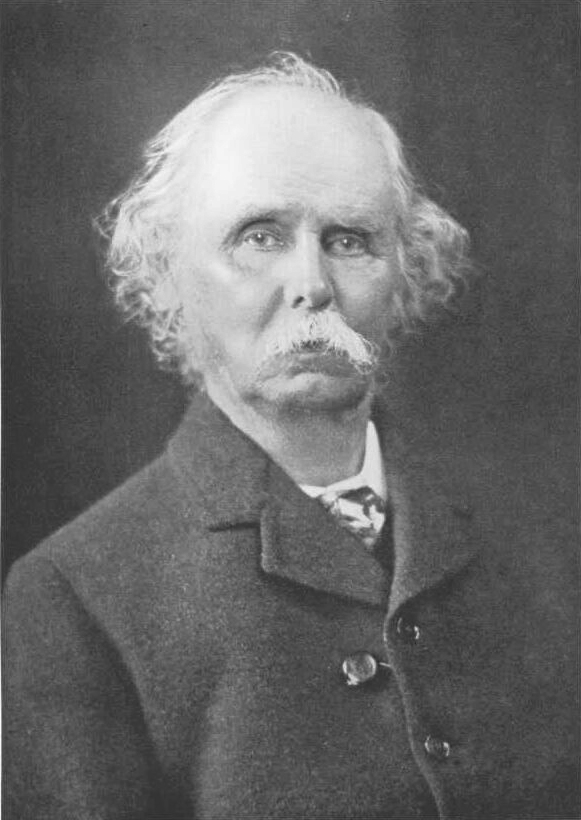
\includegraphics[width=0.5\linewidth]{img/intro/Alfred_Marshall} 

}

\caption{Image Sourced from Wikipedia.}\label{fig:intro02}
\end{figure}

The ordinary business of life:

\begin{itemize}
\tightlist
\item
  majors/minors in college
\item
  degree level
\item
  career
\item
  dating and marrying
\item
  vacations
\item
  having children or not
\item
  mortgage, renting
\item
  car payments, public transport
\item
  illness, elective surgeries
\item
  retirement, unretirement
\item
  etc, etc, etc, \ldots{}
\end{itemize}

All of these are parts of life for most of us, ordinary life.

One of the greats of modern economics, Partha Dasgupta\footnote{\url{http://www.econ.cam.ac.uk/people/emeritus/pd10000}}, writes

\begin{quote}
``These are no mere academic matters. If welfare and development economics, more generally political philosophy, are not about the circumstances in which people are born and the manner in which they are able to live and die, they are about nothing.''
\end{quote}

\begin{figure}

{\centering 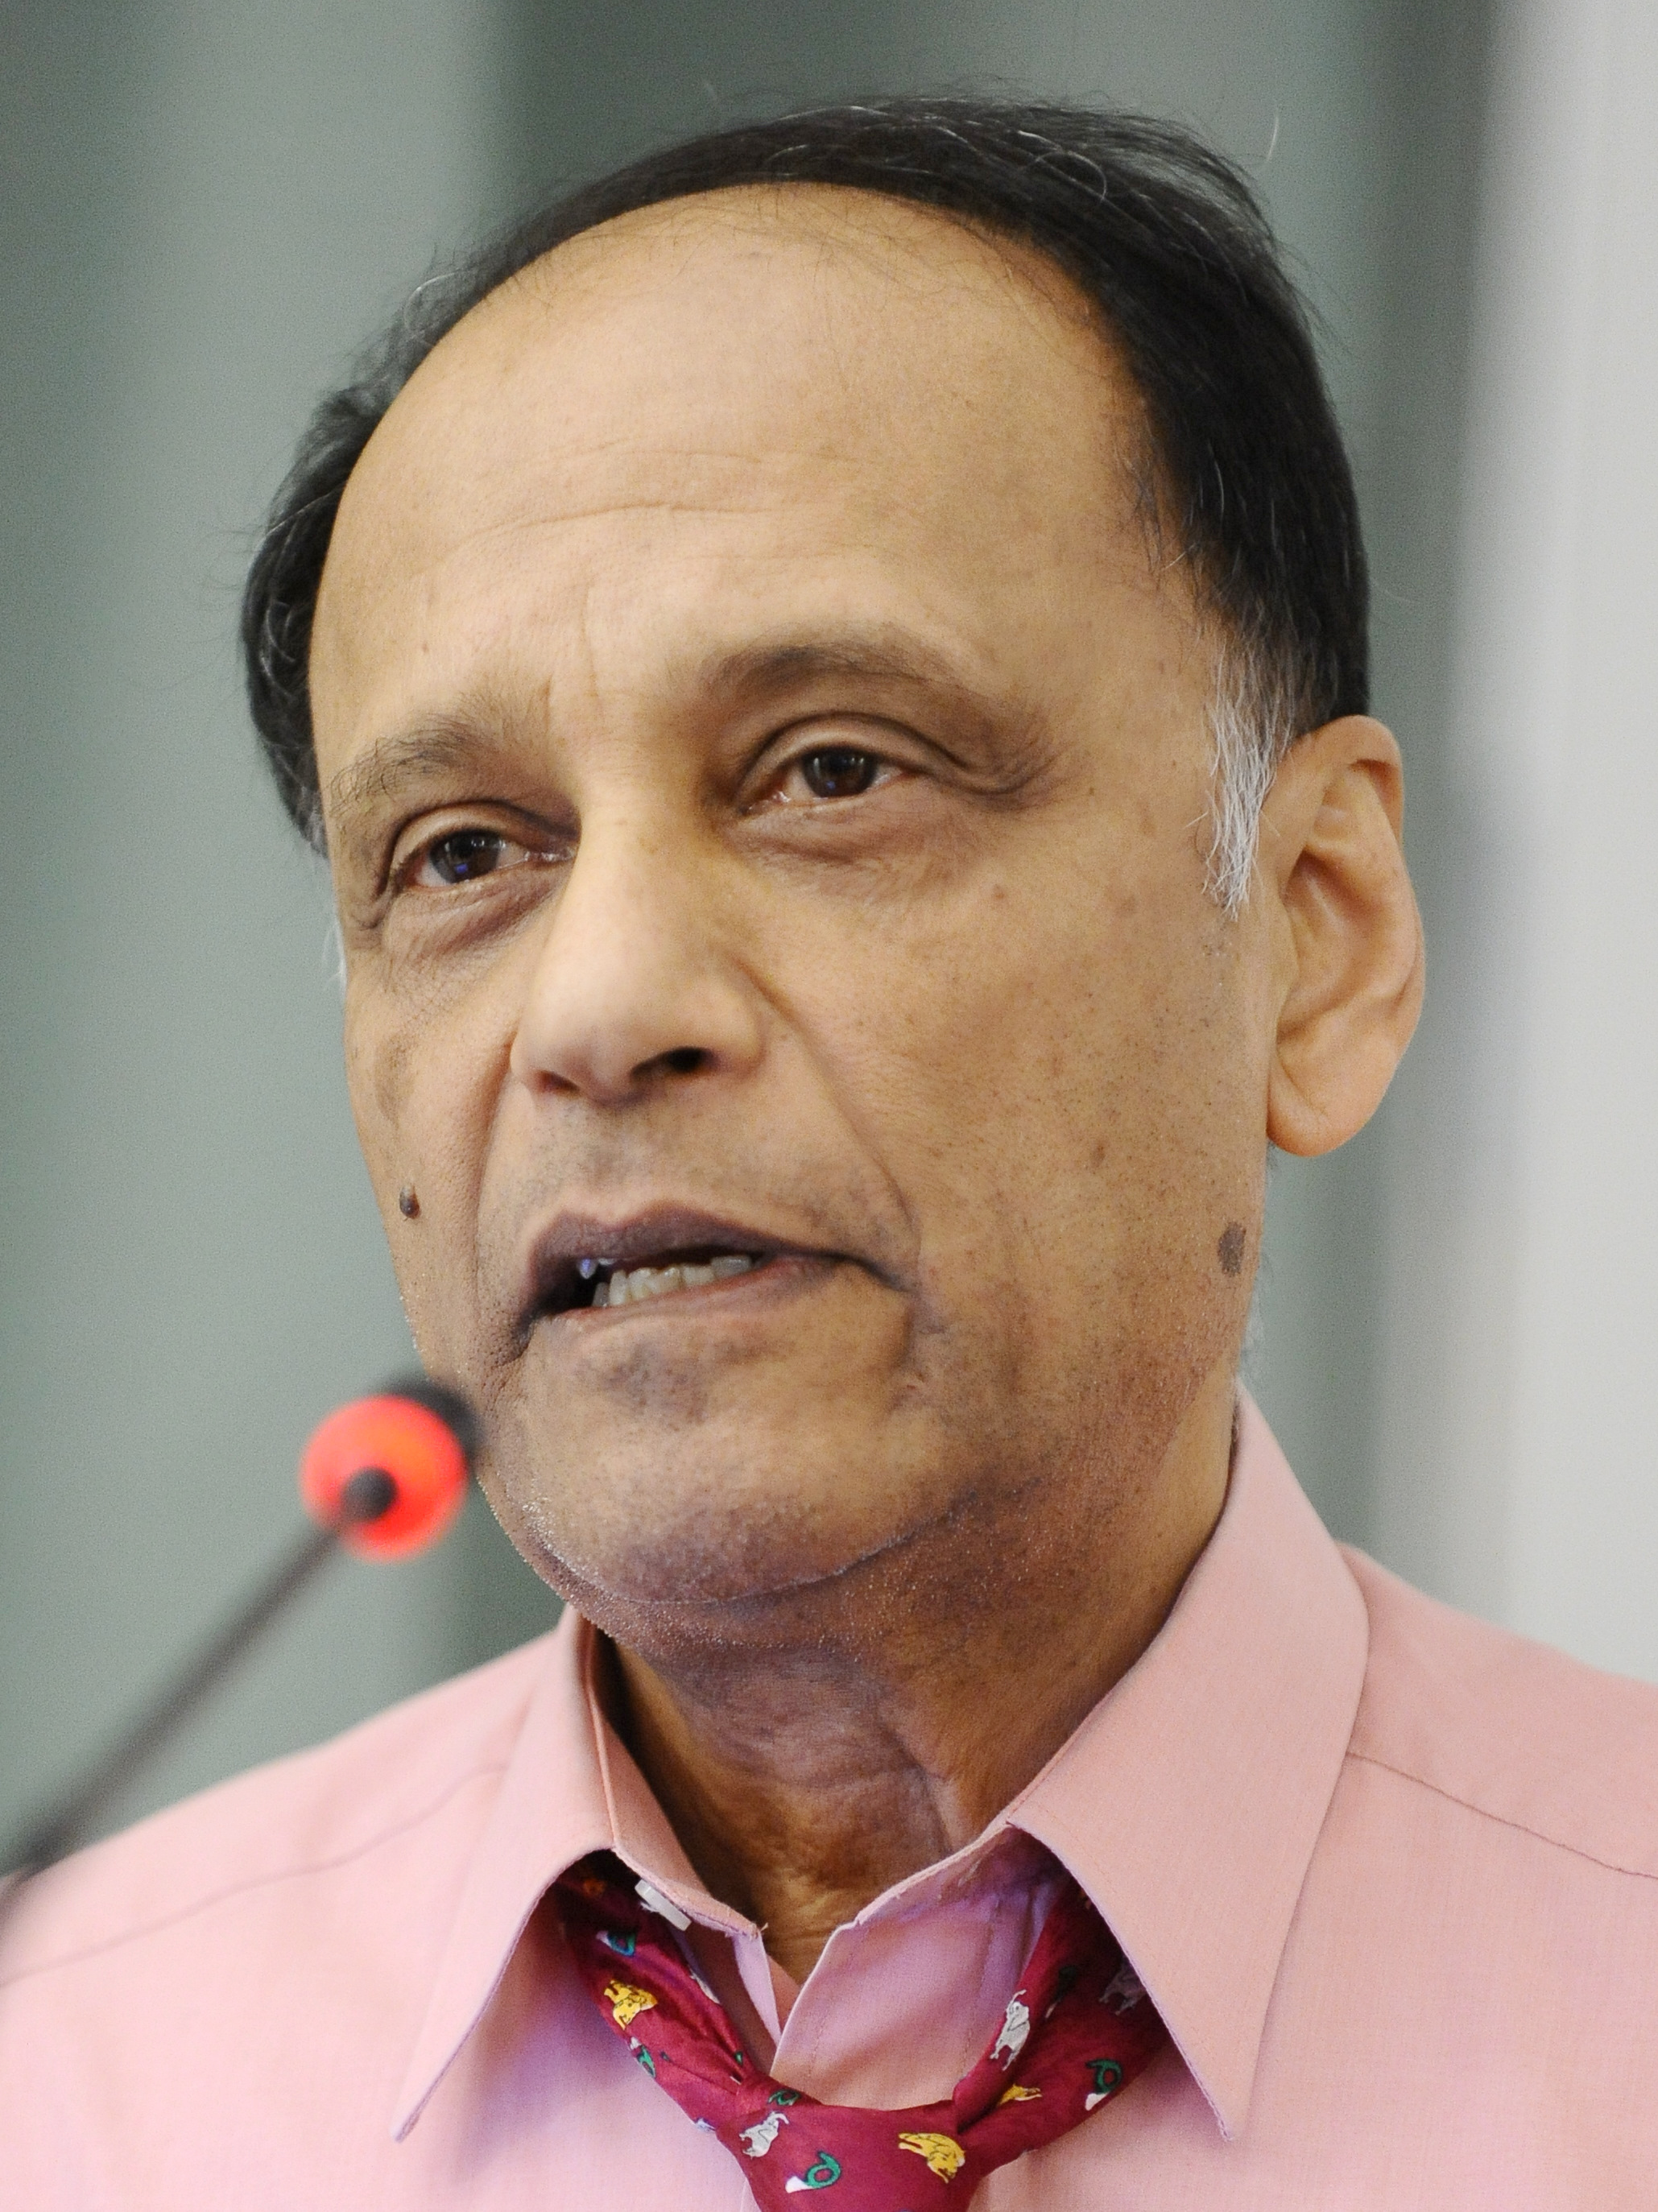
\includegraphics[width=0.5\linewidth]{img/intro/Partha_Dasgupta} 

}

\caption{Image Sourced from Wikipedia.}\label{fig:intro03}
\end{figure}

Evidently economics is about life from the moment we are born to the moment we die so anyway, with all its joys, with all its triumphs, but also with all its challenges, struggles, defeats and tragedies.

This includes the preemies that are born weighing less than 2 pounds with their and their parents' life-long struggle to flourish and to secure a comfortable life:

\begin{itemize}
\tightlist
\item
  How big are the medical bills?
\item
  Does insurance cover them all?
\end{itemize}

\begin{figure}

{\centering 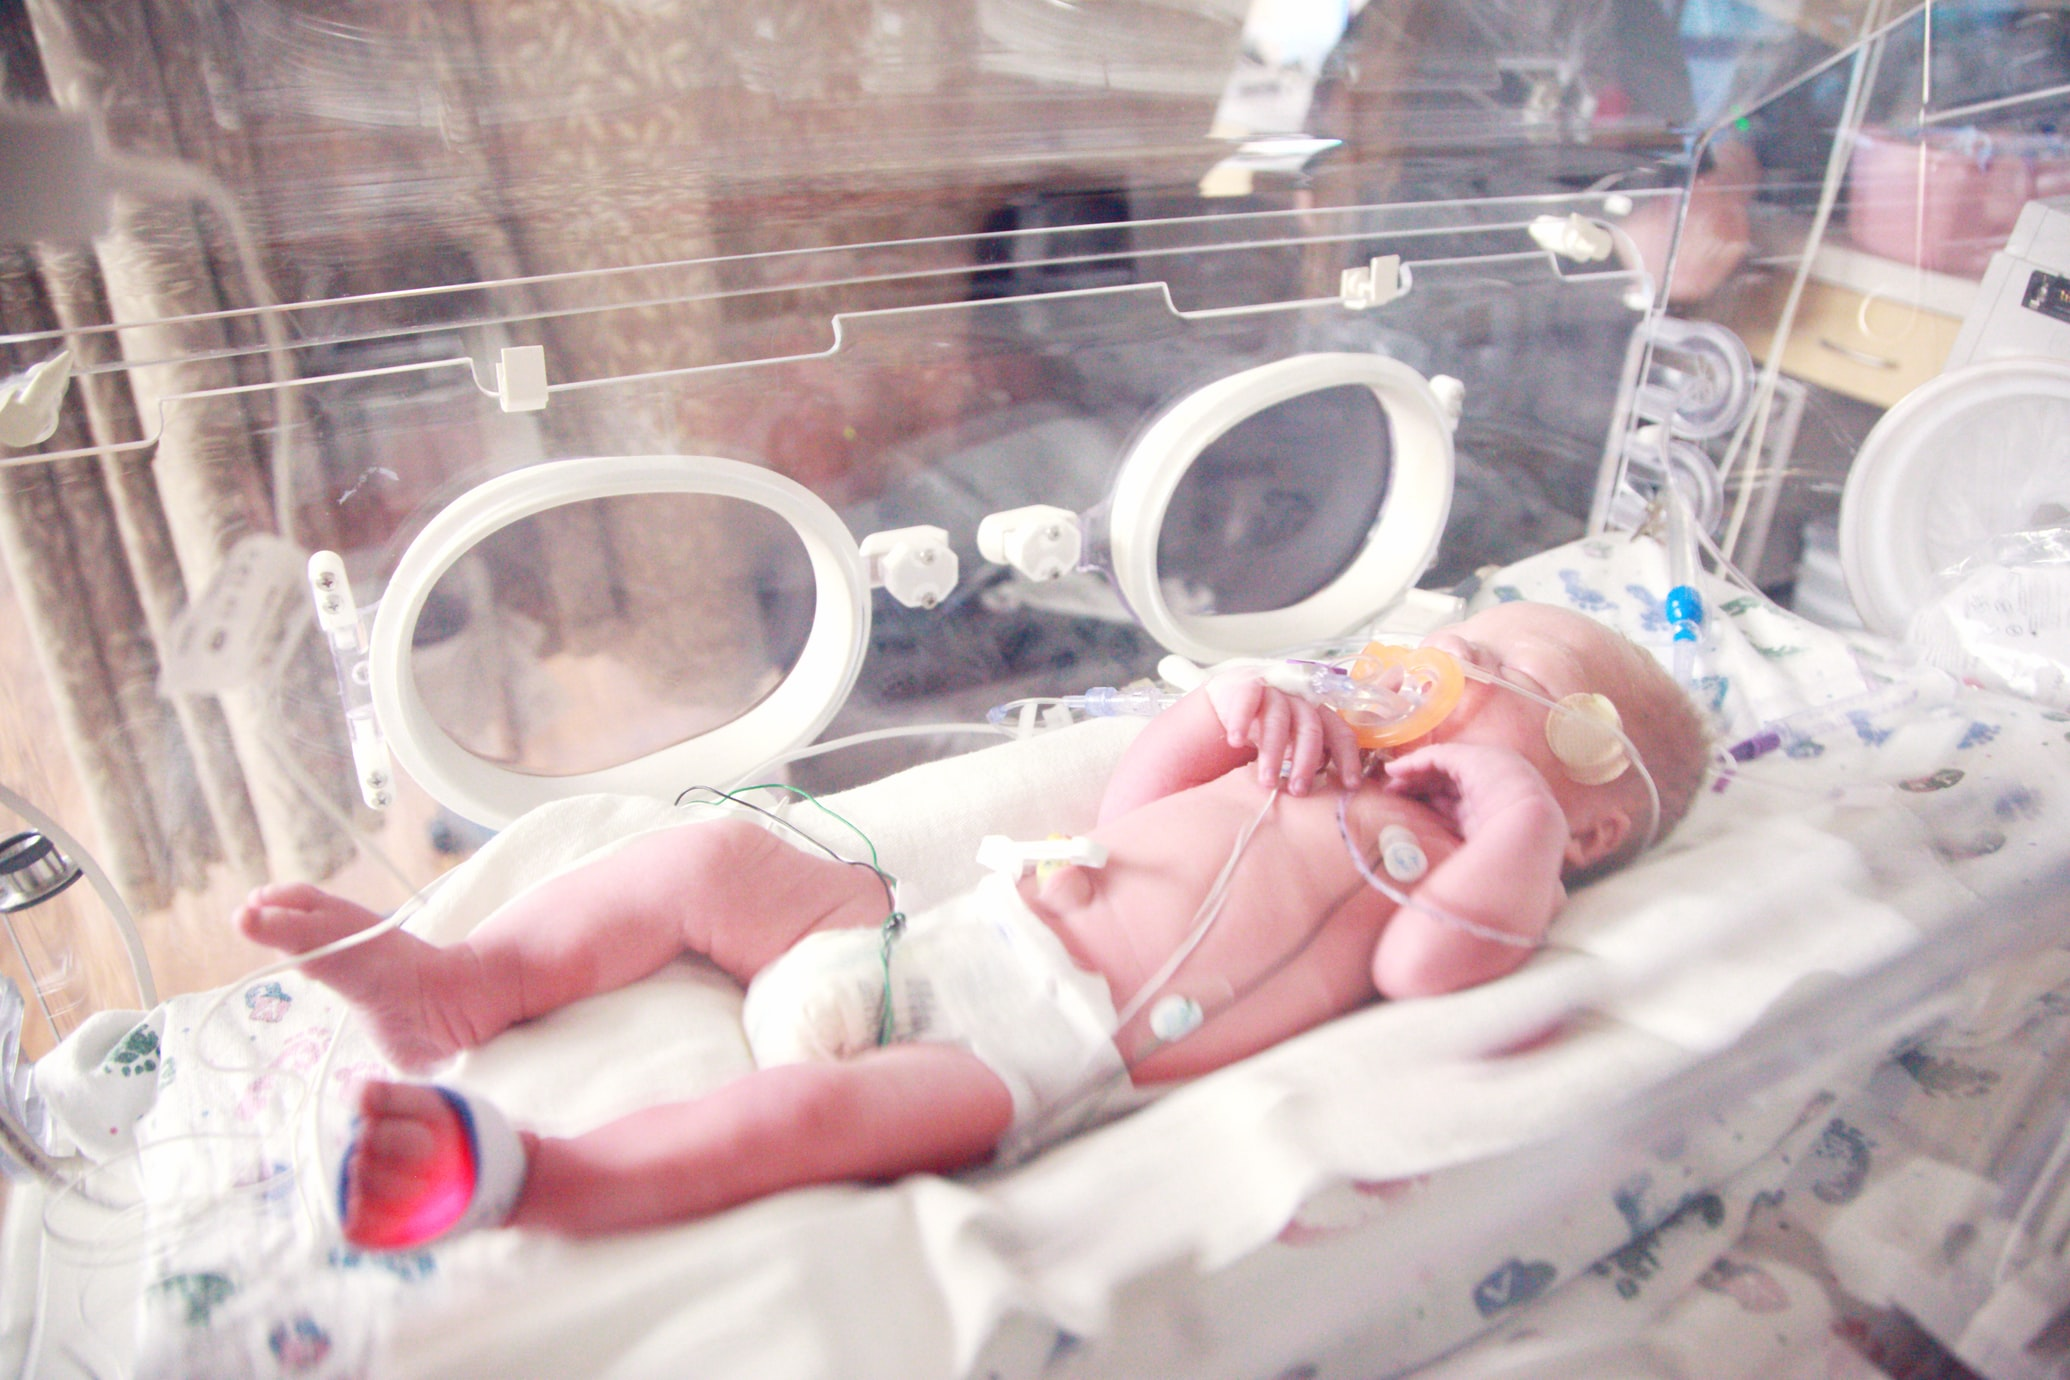
\includegraphics[width=0.5\linewidth]{img/intro/fig4} 

}

\caption{Image Sourced from unsplash.}\label{fig:intro04}
\end{figure}

This includes the child born in the wrong ZIP code area. Who is developmentally is behind at 3 years old. Who will have a hard time catching up scholastically. Who as a young adult will have difficulty making ends meet because of the poor employment prospects.\footnote{\url{https://research.upjohn.org/up_press/228/}}

This includes the child who is abused growing up. Who because of experience this recurring abuse is of higher likelihood to be a part of the prison system later in life.\footnote{\url{https://www.nber.org/digest/jan07/does-child-abuse-cause-crime}}\footnote{\url{https://www.cdc.gov/vitalsigns/aces/pdf/vs-1105-aces-H.pdf}}

This includes the young person who graduated from college with huge student debt that is impossible to be paid back and that is very unlikely to be forgiven, even in bankruptcy.

This includes the parents of young children who are torn between going to work to pay the bills and staying home with their children because there is no reliable and safe childcare during covid-19.

\begin{figure}

{\centering 
\includegraphics[width=0.5\linewidth]{img/intro/fig5} 

}

\caption{Image Sourced from unsplash.}\label{fig:intro05}
\end{figure}

This includes the retired college professor whose physician tells him:

\begin{quote}
``Walter, with your lung cancer you have 6 months to live, on the outside. Now is the time to do the things you've always wanted to do but have never done.'\,'
\end{quote}

But who, the following morning, gets ready to go to his office, and when reminded by his wife of the physician's advice that now is the time to do the things he always wanted to do, replies:

\begin{quote}
``That is exactly what I'm doing. I am doing what I've always wanted to do. I am going to the office to do my work.'\,'
\end{quote}

This includes the mother from Nicaragua, Guatemala, or Honduras, who flees with her children north, to what she thinks is a safer place for her children knowing full well the meaning and implications for her of the term ``cuerpomatic'\,'\footnote{\url{https://www.americasquarterly.org/blog/rape-another-threat-on-migrant-womens-journey-north/}}.

This includes things like assortative mating or ``like marries like.'' Tall men/women tend to marry tall women/men. Another way of saying this is: The height of married couples is positively correlated. Highly educated women/men marry highly educated men/women. The level of education of married couples is positively correlated. The level of incomes are positively correlated.\footnote{\url{https://www.nber.org/system/files/working_papers/w19829/w19829.pdf}} It was not always like this.

This includes all those people who suffer from kidney failure, who are waiting for a transplant kidney, who may or may not get one. In this country, about 13 people die per day, because there are no transplants available.

\begin{figure}

{\centering 
\includegraphics[width=0.5\linewidth]{img/intro/fig6} 

}

\caption{Image Sourced from unsplash.}\label{fig:intro06}
\end{figure}

Most textbooks define economics to be the study of the allocation scarce resources. A resource here is simply a means, something that is useful. Useful for a purpose. We usually assume that people have goals and that they will try to achieve these goals. But there are constraints that stand in the way.

Money is resource that allows us to buy stuff. For most of us money is scarce, our budgets are limited. Therefore, we must make choices:

\begin{itemize}
\tightlist
\item
  The fancy car or a super vacation?
\item
  Paying the utility bill or paying the medical bill?
\item
  A fancy wedding or a dream house?\footnote{\url{https://www.netflix.com/title/81113929}}
\end{itemize}

\begin{figure}

{\centering 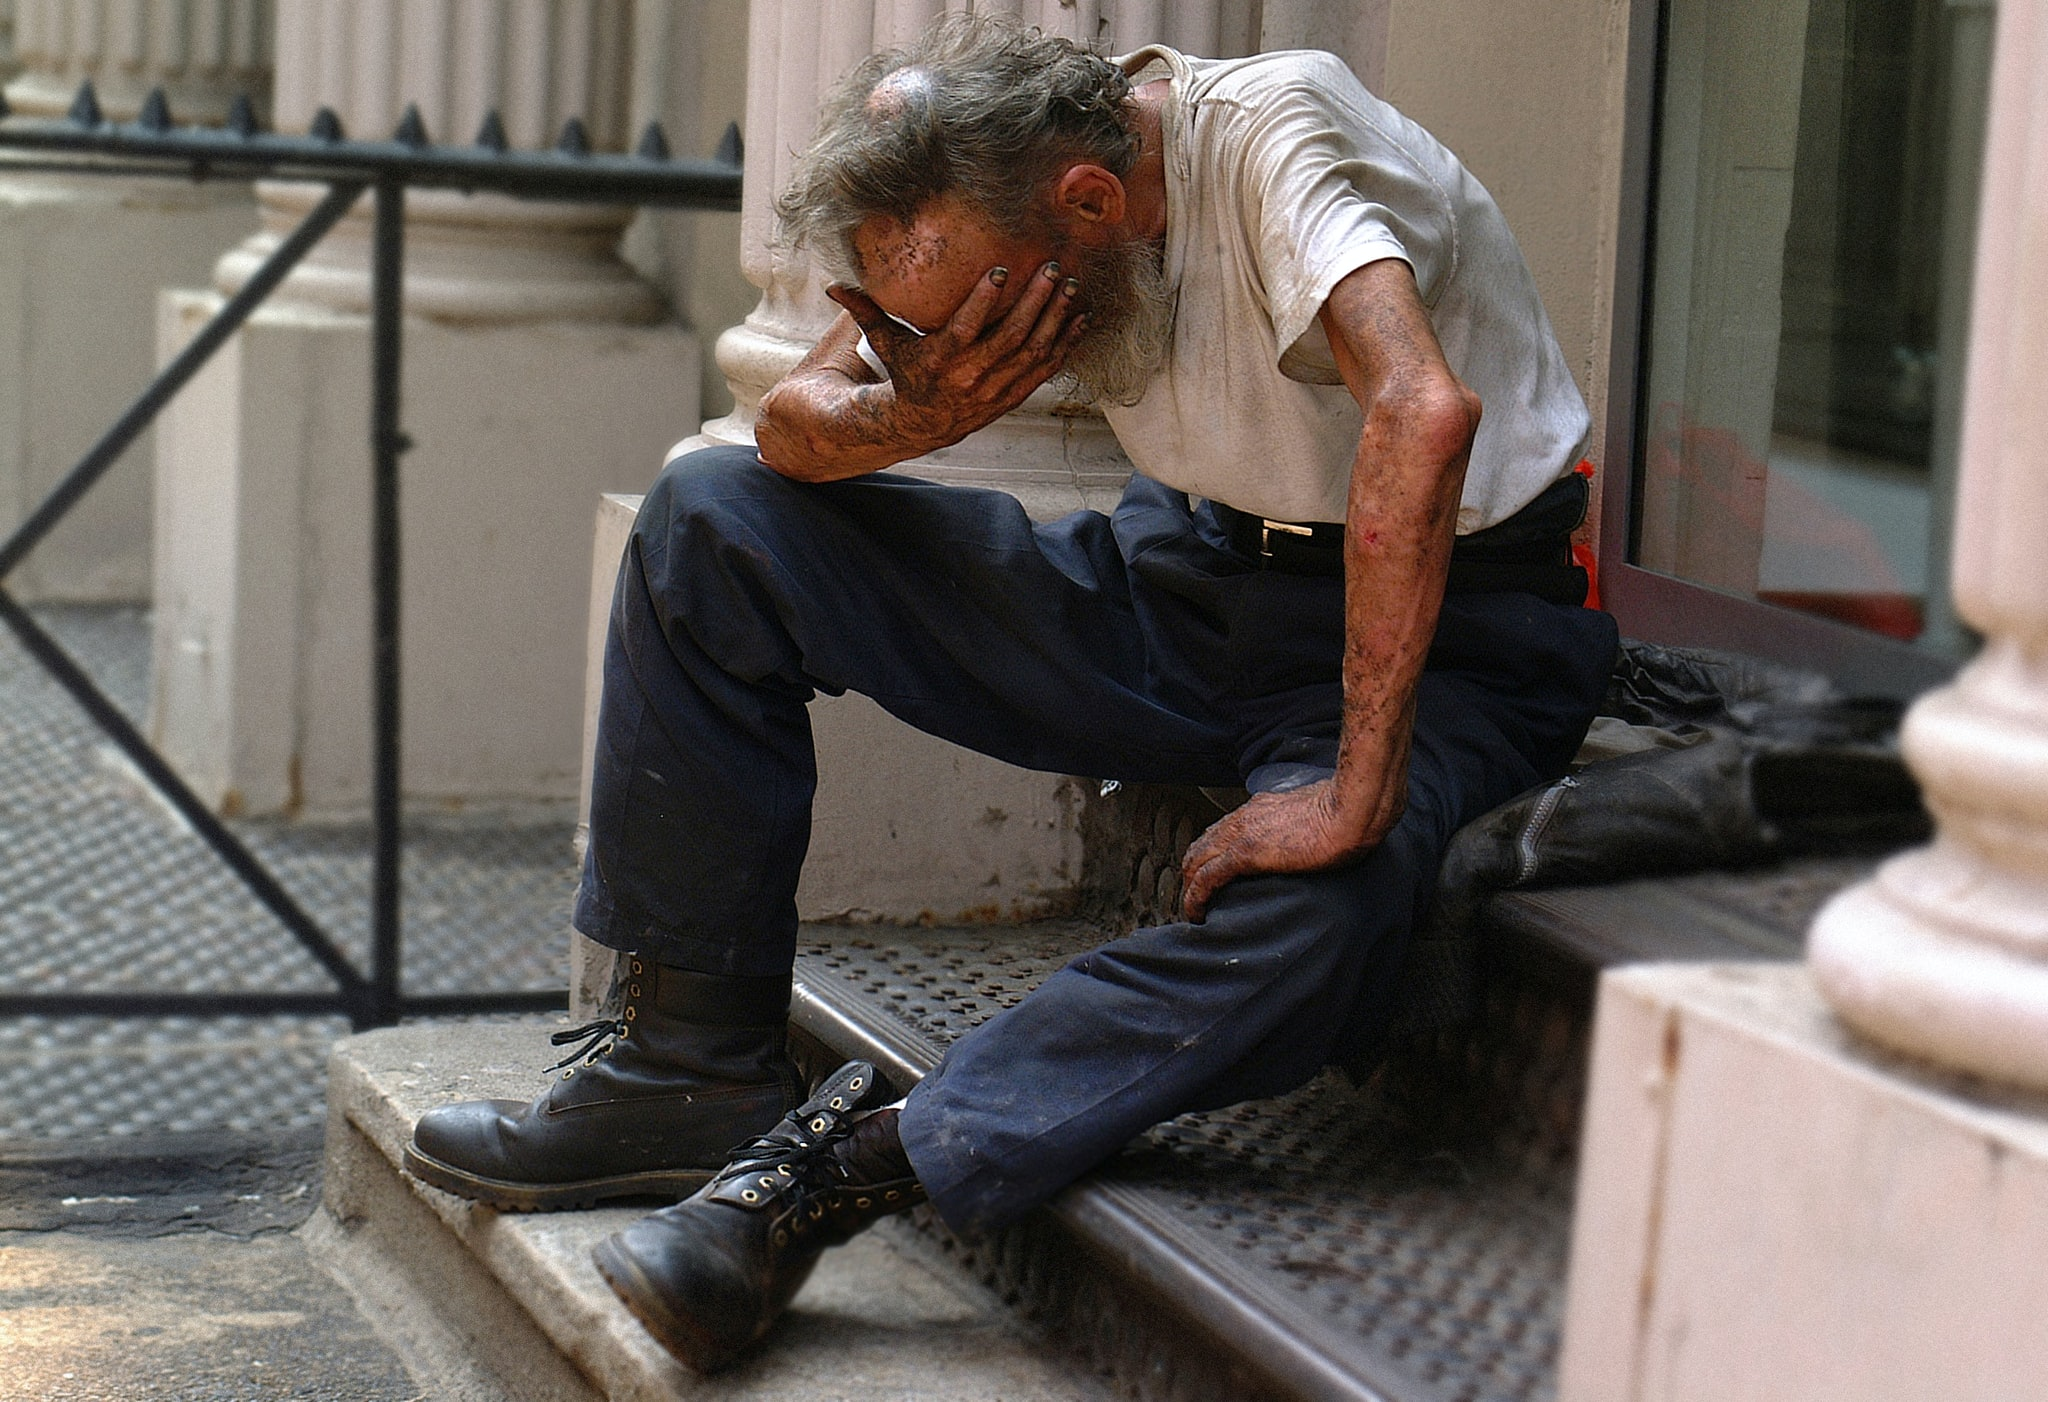
\includegraphics[width=0.5\linewidth]{img/intro/fig7} 

}

\caption{Image Sourced from unsplash.}\label{fig:intro07}
\end{figure}

Time, perhaps our most valuable resource, is also scarce. You will surely notice this, as many have before you, during finals week. You will wish that there were five or six extra hours in each day.

Bandwidth, our ability to compute, to calculate, to process information, to decide rationally, is surely limited and many of us wish that our bandwidth were much, much bigger.

\hypertarget{what-is-economics-good-for}{%
\section{What is Economics Good For?}\label{what-is-economics-good-for}}

First and foremost economics is a social science. We would expect economics to be good and useful in explaining behavior. When we look around, there are all kinds of interesting observations that we would like to explain. And economics can help us go a long way towards providing explanations for all kinds of behavior. Some examples we might have insight to:

\begin{itemize}
\tightlist
\item
  Why did grocery stores run out of toilet paper at the beginning of the covid-19 pandemic?
\item
  Why did women suffer more than men from the covid-19 induced epidemic when normally in other recessions men tend to suffer more employment losses than women?\\
\item
  Why are Dutch women taller than American women?
\item
  Why do women when they buy a house from a man pay a higher price than a man and when they sell a house to a man they get a lower price than a man?
\item
  Why did the price of bicycles rise during the covid-19 recession?
\item
  Why did the price off used cars rise during the covid-19 recession?
\item
  Why has the labor force participation of males been dropping for the last 20 or so years?
\end{itemize}

The question is always:
Why? Why? Why?

Perhaps we can spend a little bit of time thinking about the following three examples of observations and ask why did these things happen?

\begin{itemize}
\tightlist
\item
  In Maine in the 1800 Lobster was used commonly to feed prisoners and it was used commonly for fertilizer on the fields. Why?\\
\item
  In a recent 5K race in Bloomington Indiana there were participants in basically all age groups from age 16 all the way up to age 80. this was true for both men and women with one exception. in the category Between age 30 and 35 there was not a single female participant. Why?\\
\item
  According to some reports from field workers In a refugee camp for the Rohingya in Bangladesh There were children older than five years of age and younger than 2 but there were no children between the ages of 2 and 5. Why?
\end{itemize}

We will see how economics can provide answers too many of these why? why? why? Questions.

Economics can also provide answers to questions like what are the underlying assumptions that some individuals make under which their behavior might be rational?

If we consider a CEO who believes they are running late to a meeting for a merger worth millions of dollars. We might think driving at very high speed under these circumstances actually makes a lot of sense. It is the rational thing to do.

On May 25, 2020, Amy Cooper, a white woman, let her dog off its leash in Central Park. Christian Cooper, a black male who was in the park watching birds asked her to leash her dog back up. Amy Cooper called the police alleging an ``African American man'' was threatening her.\footnote{\url{https://www.nytimes.com/2020/07/06/nyregion/amy-cooper-false-report-charge.html}}

Under what assumptions is the behavior of Amy Cooper in Central Park rational? \href{https://www.ncronline.org/news/opinion/assumptions-white-privilege-and-what-we-can-do-about-it}{This article} digs into this. Rationality here and in the rest of these notes means: Our actions are guided by a particular purpose or goal, taking into consideration all constraints and all relevant information. Bryan Massingale in the article below list many assumptions under which Amy Cooper's behavior in Central Park is actually rational. Her actions seem to make sense under the assumption that her word as a white female would have more weight than the word off a black male. Since she must have thought that any police officers, not a particular police officer, summoned by her would give more credibility to her word than to the black male, she must have believed and hoped for what we would call systemic racism. Her actions make sense, her actions are rational, if she believes in systemic racism.

The second thing economics is good for is to evaluate policies. Policies are just the things institutions (or government in particular) do. The federal government determines spending on defense and Medicare. It regulates immigration to this country. The state government chooses educational policies and whether to legalize weed. A local government decides to fund public parks and bicycle paths. A country club determines the rules for the use of a golf course. A faith organization chooses particular youth programs. A corporation chooses particular HR policies.

In each one of these cases we want to know:

\begin{itemize}
\tightlist
\item
  Does the policy work?
\item
  Is it a good policy?
\end{itemize}

We want to be able to hold public officials accountable for the policies they pick. In order to be able to do, we need to be able to figure out how people respond and react to these policies.

This leads us to a subject that is covered in the opening chapters of all introductory economics textbooks:

\textbf{The law of unintended consequence}

\hypertarget{unintended-consequences}{%
\section{Unintended Consequences}\label{unintended-consequences}}

The law of unintended consequences simply states that when a policy is changed, people will respond to that policy change, and frequently in ways that are difficult to forecast by the policy maker. Of course, the more careful the policy maker thinks about possible responses of people to the change in the policy, the fewer surprise responses to the policy there will be. But it is a testimony to human ingenuity and creativity that even with the best intention the best laid plans of mice and men often lead to disastrous outcomes. My guess is that such adverse responses to policy changes will never be eliminated, even after the most careful analysis of the proposed policy change.

It should not be a surprise that bad people will respond to changes in a policy. People simply do what they believe is in their best interest and when incentives change, chances are their behavior will change as well.

If I announce that in this class there will be a final exam that is comprehensive, that is the hardest exam on campus with a pass rate off only 30\%, there are a variety of possible reactions to this kind of an announcement. Some students will decide to study harder, some students might get a tutor, some students might decide to come to office hours more frequently. Some students might just give up, drop the class and wait until that class is offered by a different faculty member who has easier exams. This is just incentives at work. But we have to acknowledge that the different students will respond in different ways and it is just extremely difficult to predict the behavioral response a particular student.

There are some interesting responses to changes in government policy.

\hypertarget{unintended-consequences-examples}{%
\subsection{Unintended Consequences Examples}\label{unintended-consequences-examples}}

\textbf{(Epidemics I)} I heard of a convenience store in Virginia that had attached to it a video arcade with a separate entrance. During covid-19, the convenience store was declared essential and allowed to stay open, the video arcade shut by order of the government. How did the owner of the convenience store and the video arcade respond to this government policy? He simply moved some of the video games into the convenience store, thereby increasing the density of customers in the store and the therefore the risk of infection of customers.

\begin{center}\rule{0.5\linewidth}{0.5pt}\end{center}

\textbf{(Epidemics II)}\footnote{\url{https://crofsblogs.typepad.com/h5n1/2020/05/trumps-europe-travel-ban-triggered-covid-19-spreadin-the-us.html}} On March 11, 2020, President Trump announced a travel ban from most countries in Europe to be effective March 13th and to last 30 days.

\begin{itemize}
\tightlist
\item
  If you are an American traveler in Europe, how would you respond to this announcement?
\item
  If you are an American tourist in Europe, how would you respond?
\item
  If you are an American on business in Europe, how would you respond? - Or, if you are an American student on an exchange program in the affected European countries, how would you respond?
\end{itemize}

Regardless of your original plans for your return trip, you might well conclude that the best course of action for you is to hightail it home as quickly as you possibly can.

Evidently, many Americans decided that this was indeed their best course of action, so they change their plans and return home as quickly as possible. As a consequence, American airports on March 12 and 13 were overcrowded, contributing to the further spread of the virus. Perhaps this crowding might have been avoided to some degree buy more carefully planning the return flights and spreading out over time the arrival of these flights into international American airports.

\begin{center}\rule{0.5\linewidth}{0.5pt}\end{center}

\textbf{(Work Incentives)} During the financial crisis off 2008 and 09 the governments in many affected countries designed rescue packages to bailout banks, at least the largest banks. Some of these rescue packages contain explicit caps on bonuses for banking executives. If the government imposes caps on those bonuses, how might banks respond to such limitations? Well, if I cannot reward my employees through higher bonuses, I can still reward my employees by increasing their base salaries. To the extent that the bonuses are used to reward exceptionally good performance and thereby provide incentives for such exceptionally good performance, this cap on bonuses seems to have one adverse effect: weaker incentives for exceptional performance. Not sure if that is what you want.

\begin{center}\rule{0.5\linewidth}{0.5pt}\end{center}

\textbf{(Health)} Imagine you are concerned with excessively long waiting times at emergency rooms in the hospitals in your state. Suppose you want to design a scheme that rewards hospitals to decrease those waiting times. So, you collect the data on average waiting times in these emergency rooms and then you design rewards for those hospitals who reduce the waiting times the most. If you measure waiting time from the moment the patient comes through the door to the time the patient is treated, how might hospitals actually respond to this new policy?
Hospitals might ask the ambulances to wait in the hospital parking lot. Surely this is not a desired outcome.

\begin{center}\rule{0.5\linewidth}{0.5pt}\end{center}

\textbf{(Education)} Supposed you want to reward teachers for better performance of their students on standardized tests. Suppose the stakes, the rewards are big. How might the teachers respond to these incentives? Surely there are many possibilities.

Some teachers might better prepare their lessons.

Some teachers might spend more time with students who are struggling.

But some teachers might also provide caffeinated sugary drinks to their students the day of the test to get a short time boost in attention and concentration to improve their performance. I suspect the dentists will love this.

Or, and this is an extreme case, some teachers might actually be induced to cheat on behalf of their students. One example of teachers engaging in such cheating is documented in the first book Freakonomics.

\begin{center}\rule{0.5\linewidth}{0.5pt}\end{center}

\textbf{(Gender)}\footnote{\url{http://ftp.iza.org/dp9904.pdf}} Family leave policies are intended to allow moms and dads to spend quality time with their new-born babies. In many places/organizations there has been a gradual shift from no leave, paid or unpaid, to maternity leave for the mom to family leave for both mom and dad, when a baby is born. In some organizations there is still no maternity or family leave policy in place and women have to take sick days or personal days to deliver their baby. At a typical university maternity or family leave is ties to ``stopping the tenure clock.'' Stopping the tenure clock simply means, that mom and/or dad have extra time, often one year, to be considered for tenure. Tenure basically ensures lifetime job security. Its is a BIG deal.

Allowing dads time off and stopping the tenure clock for dads as well as for moms is often seen as a great equalizer of men and women, dads and moms. After all, now dad can spend time with his baby as well. What could possibly be or go wrong with that?

The paper below shows that the policy of providing gender neutral family leave and stopping the tenure clock in a gender-neutral way, increases dad's chances of tenure by 19 percentage points and decreases mom's tenure of tenure by 22 percentage points.

So much for achieving gender neutrality!

\begin{center}\rule{0.5\linewidth}{0.5pt}\end{center}

\textbf{(Gender II)}\footnote{\url{https://www.cesifo.org/en/publikationen/2020/working-paper/caught-between-cultures-unintended-consequences-improving}} The German government passes a law that grants automatic German citizenship tights to all immigrant children born in Germany after January 1, 2000. You might think that such a law would benefit all immigrants regardless of country of origin, skin color, religion, sex, gender identity and age. Why? It is just a right. The law increases the realm of the possible. It increases opportunities. It does not take away any opportunities. What could possibly be wrong with more choices, more opportunities? So, one would be inclined to think that all immigrants would be better off and report being happier. And in that believe we would be wrong. Why? The law of unintended consequences strikes again.

Self-reported happiness declined after this law was passed for Muslim girls. Muslim immigrant girls become disillusioned. Muslim parents are less likely to help their daughters who qualify for citizenship with their homework. They are also less likely to speak German with their daughters. Muslim immigrant girls who qualify for German citizenship are less likely to self-identify as German.

The law of unintended consequences truly rears its ugly head.

None of these effects are found for Muslim boys. None of these effects are found for children of other faiths.

Why do we find these effects for Muslim immigrant girls? Parents of Muslim immigrant girls react strongly to counter effect the pull of German society to keep their daughters withing their cultural and religious traditions.

\hypertarget{exercises}{%
\subsection{Exercises}\label{exercises}}

\begin{enumerate}
\def\labelenumi{\arabic{enumi}.}
\item
  Suppose the State passes a law that allows for ``No knock warrants.'' \href{https://en.wikipedia.org/wiki/No-knock_warrant\#:~:text=In\%20the\%20United\%20States\%2C\%20a,knocking\%20or\%20ringing\%20a\%20doorbell}{See here} if you are unsure what this is.

  A. Make a list of the possible ``unintended consequences'' of this policy.\\
  B. Who would get impacted by this policy? Positively or negatively?\\
  C. How hard is it to foresee/forecast these consequences?
\item
  President Trump issued an Executive order on June 22, 2020 to severely limit H1-B and L1 visas. H1-B visas are visas issued so American companies can hire high-skilled immigrants. L1 visas allow American multinational corporations to transfer foreign managers and employees to their offices in the US.\footnote{\url{https://www.nber.org/papers/w27997}}

  A. Make a list of all the effects of this policy. Who would get impacted by this policy? Positively or negatively?\\
  B. How hard is it to foresee/forecast these consequences?
\end{enumerate}

\hypertarget{role-of-theory}{%
\section{Role of Theory}\label{role-of-theory}}

What is the role of theory in economics?

A quote by a 12th century philosopher, Peter Abelard:

\begin{quote}
``The man of understanding is he who has the ability to grasp and ponder the hidden causes of things. By hidden causes we mean those from which things originate, and these are to be investigated more by reason than by sensory experiences.''
\end{quote}

We can paraphrase this by saying: If we want to understand stuff, we ought to rely more on our brain and think more about how things might actually work, rather than collecting data with our senses.

Charles Darwin, in a letter to one of his friends expressed a similar opinion:

\begin{quote}
``About thirty years ago there was much talk that geologists ought only to observe and not theorise; and I well remember someone saying that at this rate a man might as well go into a gravel-pit and count the pebbles and describe the colors. How odd it is that anyone should not see that all observation must be for or against some view if it is to be of any service!''
\end{quote}

I interpret that last clause in Darwin's letter to mean: All observations must be used to either confirm or reject a hypothesis or theory, if the observation is to be of any use at all. That implies that theory comes first.

So, what is this thing called a ``theory?'' I will use the words: theory, model, and abstraction synonymously. A theory is a creation of our minds; it is an idea of how some part of the word operates or might operate.

The theories we use will be different in economics and in physics. Even within economics there will be different theories or models. Macroeconomists will use different models than economists who study anti-trust. The main job of a model is to help us understand how a part of the world works. Any theory or model is supposed to be useful, for understanding.

\hypertarget{abstractions}{%
\subsection{Abstractions}\label{abstractions}}

How is an abstraction useful? Suppose the job is to drive from Bloomington, IN to Martinsville, IN. We need a map to help us get there.

\newpage{}

Above we have a map. It has all kinds of information. State Forests, State Parks. Where Bloomington's airport is. County lines. If we zoom out, we get state borders, Lake Michigan, Lake Erie, etc. A whole bunch of information about Illinois. Much of this information is not relevant if the task is to get from Bloomington to Martinsville.

In order to get from Bloomington to Martinsville, not much information is needed. Most, practically all of the information above is useless and needs to be discarded. Pretty much the only information needed is illustrated below. All we need is the starting point, Bloomington, the endpoint, Martinsville, and the instructions to get on I-69 in Bloomington until the sign ``Martinsville, IN'' appears. This is really all that is essential.

Bloomington---------------------------I 69---------------------------------Martinsville

There are a few more things that one might reasonably add to our ``model'' of the relevant piece of geography. It might be useful where the gas stations are, especially the ones with clean bathrooms, and where the coffee shops are so the driver does not fall asleep. One such establishment, marked by G for gas station, is added in the model below.

Bloomington---------------------------I 69--------------------G-----------Martinsville

\hypertarget{prejudice-based-wage-discrimination}{%
\subsection{Prejudice-Based Wage Discrimination}\label{prejudice-based-wage-discrimination}}

How to find prejudice-based wage discrimination?

In this example I will try to show that economic theory can generate useful insights or knowledge. The way this works in this example is that economic theory will suggest precisely where we have to look for evidence. The issue or example that we will use here is the question:
How, if, and to what extent does racial prejudice show up in or generate wage discrimination by race?

The work in economics on racial discrimination goes back at least to the seminal work by Nobel Laureate Gary Becker from the University of Chicago.

For starters, we have to distinguish between prejudice and wage discrimination. Prejudice is an attitude, a negative attitude, a sentiment toward a particular group of people, Blacks for example. Wage discrimination is a particular outcome in labor markets that simply says comparable blacks and comparable whites earn different wage rates.
The question then is: How, to what extent, if at all, does racial prejudice determine such wage discrimination?

In order to start thinking about this issue, we will consider a very simple example. Blacks make up about 10\% off the population or the labor force. There are two distinct labor markets. In labor market 1 the population of white people exhibits basically no racial prejudice. In labor market 2, the population of white people exhibits very strong racial prejudices.

In which labor market would we expect wage discrimination by race to be strongest? Labor market 1 or labor market 2?

Without a moment's thought most of us would be tempted to say: Of course, racial discrimination higher, stronger, worse in labor market 2 than in labor market 1.

But that would be missing an element off the story that probably is very important.

Blacks will most likely know or at least have some pretty good information on where the racists live, in which labor market they operate. Why would they know this? Chances are they have experienced the manifestations of racism and through their social network this information is broadly shared.

So, to the extent that blacks have information on manifestations of racism and to the extent that they are free to move between labor markets, to choose their place of employment, they will probably move from labor market 2 two labor market 1. This is of course, holding other things equal. holding other things equal just means that in all other aspects these two labor markets are roughly comparable. They only differ in this one aspect: prejudice.

So, if blacks can move freely, relatively freely, they will choose labor market 1 over labor market 2 in which case there might be very little racial wage discrimination in labor market 2. If all Blacks where to move into labor market one, then there would be no racial wage discrimination in labor market 2 at all.

Therefore, our answer that labor market 2 will exhibit more wage discrimination than labor market 1 is probably false.

There is a \href{https://papers.ssrn.com/sol3/papers.cfm?abstract_id=1073644}{recent paper linked here}, together with a \href{https://www.youtube.com/watch?v=N38XrQ6x7ck}{short video} by one of its authors, that uses currently available data to show us exactly where and how we should look for the impact of prejudice on labor market discrimination.

We start with constructing a racism distribution. This is not just some fancy Ivory Tower notion. This distribution is firmly grounded in data. There is a data set that is widely available, called The General Social Survey, GSS, that asks questions like:

\begin{itemize}
\tightlist
\item
  How would you respond if your daughter dated a black person?
\item
  Would you vote for a black man for president of the United States if he were qualified?
\end{itemize}

Answers to questions like these can be put together to create an index of racism and then a distribution of racism in a particular locality. The figure below illustrates such an example off a racism distribution.

Some researcher suggests that in order to assess the impact of prejudice on wage discrimination one should look at a correlation between the average or median degree of prejudice and the average level of wage discrimination. They collect the best data available for the 50 States and calculate or estimate that correlation. They find nothing.

Why?

Just like in the example with 2 labor markets, Blacks will, if they can, avoid the right tail of the racism distribution. They will shift to the left as far as possible in the racism distribution.

In Wisconsin, about 6\% of the labor force is black. If they all seek employment, they would be matched with some, mostly likely white, employer. If we line up all white employers on a racism distribution, with the least racist employers on the left and the most racist employers on the right, then black workers would seek employment as far away from the most racist employers as possible. Black workers would go to the left of the racism distribution as much as possible. Since Blacks in Wisconsin make up 6 percent of the population, these 6 percent would then be seeking employment from the 6 percent of the least racist employers. Since Blacks are seeking employment as far to the left tail of the prejudice distribution as possible, then it is the 6 percentile of the prejudice distribution that matters for wage discrimination. Not the average, not the median. The 6 percentile.

In Mississippi, about 34\% of the labor force is black. In Mississippi, wage discrimination is determined by the 34th percentile of the prejudice distribution. Not the average, not the median, not the 6th percentile. The 34th percentile.

So far, we have not looked at any data; so far this is all theory.
What is in the data?

When you look for the connection between prejudice and wage discrimination by looking at averages you find nothing.

But when you look for it in the way suggested by the theory, the 6th percentile of prejudice distribution in WI, the 34th percentile in MS, then BINGO! There it is, clear and significant evidence linking prejudice to wage discrimination. You just need to know where to look. Theory helps.

\hypertarget{dealing-with-data}{%
\section{Dealing with Data}\label{dealing-with-data}}

\hypertarget{empirical-regularities}{%
\subsection{Empirical regularities}\label{empirical-regularities}}

First of all, we note that we are more interested in empirical regularities than in singular observations. Jennifer is 5'4'' is an example of a singular observation. That is only one observation. Dutch women are tall is an example of an empirical regularity. This observation is more general. We would find this if we looked at a sample of women from Amsterdam, from Rotterdam, from The Hague, etc.

Rich people live longer than poor people.

This is a fact, in Indiana, New Jersey and in Kentucky. It is also true in France and in Japan.\footnote{\url{http://www.equality-of-opportunity.org/assets/documents/healthineq_summary.pdf}}

The sex ratio in the US is 1.04. The sex ratio is the ratio of the number of women to the number of men. For each 100 men in this country there are 104 women. If you look up this ration by State, there is some variation. For most states, there are more women than men. But there are exceptions. In some Western states, there are more men than women. These exceptional states include Alaska, Montana, Wyoming. You may want to ask why there are such large differences in sex ratios across the 50 States.

Numbers: Big or small?

One of the important issues we have to discuss is: Are numbers big or small. This is especially true when we are talking about dollars, taxes, expenditures, the size of government programs.

\hypertarget{examples}{%
\subsubsection{Examples}\label{examples}}

\textbf{(Earthquake Relief)} After the Haiti earthquake in 2010, the US government committed \$100 million in earthquake relief. Big number, small number? It might look like a big number. But when you consider that there are over 300 million Americans, we realize that each of us gave about 30 cents, which looks miserly. Of course, this does not include private charitable contributions.

\begin{center}\rule{0.5\linewidth}{0.5pt}\end{center}

\textbf{(Apollo Mission)} The cost of the Apollo mission which ultimately landed a man on the moon has been estimated to be about \$150 billion, in 2019 dollars. In 2019 the White House made a request to combat deaths from illicit opioid abuse to the tune of \$7 billion. In 2018 over 67,000 people dies from opioid overdoses. Is \$7 billion a big number or a small number?\footnote{\url{https://www.whitehouse.gov/briefings-statements/white-house-seeks-billions-record-investments-stop-drug-epidemic/}}

\begin{center}\rule{0.5\linewidth}{0.5pt}\end{center}

\textbf{(Vaccine R\&D)} According to an article in The Economist, August 8-14, 2020 world- wide spending on research for a Covid-19 vaccine was about \$10 billion. Sure sounds like a heck of a lot of money. But. Just in the US, the number of people who have died, at that time, was about 100,000. The value of a statistical life\footnote{Kip Viscusi \url{https://law.vanderbilt.edu/bio/w-kip-viscusi} pioneered the research on the value of a statistical life.} in the US for the median age American is about \$10 million. Since Covid-19 takes mostly older people we might use \$5 million for the value of an older statistical life. The typical failure rate in late stages of vaccine trials is about 20\%. Multiplying the value of an older statistical life by the number of Americans who dies because of Covid-19 we get:

\$100,000 \times 5 \times 1,000,000 = \$ 500 billion

Covid-19 does not only kill Americans. And now we know that the death toll is much higher. Should we have spent more on vaccine research in 2020?

\hypertarget{correlation-vs-causation}{%
\subsection{Correlation vs Causation}\label{correlation-vs-causation}}

This distinction is crucial. Knowing whether 2 variables are correlated is useful, but it is not enough. In order to make any kind of policy decision we must know causation. Correlation only tells us about a statistical relationship. Two variables may be positively correlated or they may be negatively correlated. Suppose variable X is positively correlated with variable Y. Then if X is large (small), then Y is large (small) as well. If the two variables X and Y are negatively correlated, that means that If X is large (small), then Y is small (large). Of course, there is also the possibility of no correlation.

My typical calorie intake is positively correlated with my body weight.

The time students spend studying for Finite Math exams may be negatively correlated with the grades in English classes.

Whether students are vegetarians or not is (I suspect) not correlated with their grades in introductory History classes.

We can think of these correlations as patterns in the data. They tell us nothing about causation.

Causation is an altogether different story. Causation means that one event leads to another. The event ``An increase in the price of socks,'' will lead to the event ``I buys fewer socks.'' We will talk about this at some length in this class.

The event ``90 percent of Americans getting the Covid-19 vaccine'' will lead to the event ``Americans achieve herd immunity.''

The event ``Driving like a maniac on the interstates'' leads to the event ``The probability of fatal car crashes rises.''

There are lots and lots of examples like this. We need to be able to infer causality if we want to have any hope that the policies we pick actually make things better.

If two variables, X and Y, are positively correlated, there are several possibilities concerning causation:

\begin{enumerate}
\def\labelenumi{\arabic{enumi}.}
\tightlist
\item
  X could cause Y: an increase in X could cause an increase in Y. An improvement in nutrition in childhood causes an increase in adult height. There is no way adult height could influence the quality of childhood nutrition.
\item
  Y could cause X: an increase in Y could cause an increase in X.
\item
  X could cause Y AND Y could cause X: You study hard for your econ class and as a consequence you do well in the class. And: Since you do well in your econ class, you like econ and therefore you study harder. The hard part might be to find out which effect is stronger.
\item
  X does not cause Y, nor does Y cause X. But there is another variable, Z, that causes both X and Y.
\end{enumerate}

In order to tease causation out of the data, we try to create what we call \textbf{a parallel universe.}

The point of this parallel universe is to look at two cases, two ``universes'' that are equal in all aspects except one aspect, the aspect we want to study.

\hypertarget{examples-1}{%
\subsubsection{Examples}\label{examples-1}}

\textbf{(Stand Your Ground)} Suppose I want to study the effect of the Florida ``stand your ground law'' on homicides in Florida. Then I will collect all kinds of data for Florida. And I will collect the same kind of data in similar states. It would make little sense to compare Florida to Norway. But comparing Florida to states with similar income distribution, similar ethnic composition, similar poverty rates, similar age distribution makes sense. Like Georgia, Alabama, Arkansas.

Then we can compare homicide rates in Florida to those in other states that did not pass stand your ground laws. That is one difference we can exploit for our analysis. The other difference we can exploit for our analysis is to what happened to the trend in homicides before and after the law was passed.

The conclusion that emerges in this case is quite shocking: It appears that the stand your ground law has caused an INCREASE in homicides.\footnote{\url{https://jamanetwork.com/journals/jamainternalmedicine/fullarticle/2582988}
  For more comprehensive evidence, see
  \url{https://www.rand.org/research/gun-policy/analysis/stand-your-ground/violent-crime.html}}

\begin{center}\rule{0.5\linewidth}{0.5pt}\end{center}

\textbf{(Gender II Revisited)}In the Gender II example in the Law of Unintended Consequences examples above, how could the researchers ``establish'' or ``find'' a parallel universe? Sometimes you are just lucky. The law applied to all immigrant children born after January 1, 2000. The law separates those immigrant children born before that date from those born after that date. Children borne 6 months before and children borne 6 months after will be in the same school grade. They will be very, very similar in all or at least most other aspects. The fact that the law kicks in January 1 is very fortuitous for researchers. It creates almost ideal conditions to have a treatment group and a control group. Having a treatment group and an identical control group is what we mean by having ``a parallel universe.''

\begin{center}\rule{0.5\linewidth}{0.5pt}\end{center}

\textbf{Plastic Bag Ban} In 2015, the City of Chicago banned all single use plastic shopping bags that were less than 2.25 mils thick. All other bags were unregulated. What are the consequences of this ban?

Short answer: Stores responded by using bags that are still made of plastic and that are thicker and therefore use MORE plastic. Another unintended consequence.

Unintended consequences seem to be everywhere.

How would we know? How can we infer causality? Where are the parallel universes? Where are treatment and control groups?

The researchers reasoned that stores just inside city limits ought to be very similar to store just outside if city limits in the suburbs. The researchers also reasoned that shoppers just inside the city limit are very similar to shoppers just outside the city limit. So, data from just outside the city limit can serve as a parallel universe to what is going on inside the city limit.

There is more: Stores and shoppers just before the ban and just after the ban are going to be very similar. So, in addition to the comparison of inside and outside the city limit we have the comparison of just before and just after the ban. Looking at these two comparisons allows the researchers to nail down the effect of the ban: Disposable bag use remained very high. Many grocery stores just used bags that were just thick enough to be above the limit.\footnote{\url{https://www.nber.org/papers/w28499}}

\begin{center}\rule{0.5\linewidth}{0.5pt}\end{center}

\textbf{(Health Effects of Lead)} How damaging to your health is lead? This is a big question. Most rich countries have tried to eliminate lead from gasoline and from paint. Lead is often still found in drinking water. How does lead get into your drinking water? Through the lead pipes.\footnote{\url{https://www.economist.com/united-states/2021/04/17/replacing-lead-pipes-a-newark-success-story}}

We can narrow down the question a bit: How damaging to your baby's health is lead from drinking water?

The paper below provides an answer by consider a natural treatment and control group, or, in our language, a parallel universe. We find the parallel universe in Newark, NJ. The city was served by two different water treatment plants, with the service boundary of the two plants being basically an arbitrary line running across the city. An accident (bad decision?) in one treatment plant caused excessive corrosion and, as a consequence, excessive exposure to lead in one part of the city. This excessive exposure to lead increased the probability of low birthweight babies by between 1.4 and 1.9 percentage points. This is an increase of between 17 and 22 percent.

Exploiting such parallel universes can, evidently, be quite useful.\footnote{\url{https://www.nber.org/papers/w27996}}

\hypertarget{glossary-of-terms}{%
\section{Glossary of Terms}\label{glossary-of-terms}}

\textbf{Causation:} one event leads to another or that a change in one variable leads inexorably to a change in another variable.

\textbf{Correlation:} describes the linear relationship between two variables. It is normalized to take values between +1 and -1. This is only a description of the relationship between two variables. It has no implications for causality.

\textbf{Constraint:} a limit on what is possible. Eg: financial, physical, emotionally, etc.

\textbf{Law of Unintended Consequences:} any action, any change in a policy or in a rule is bound to have consequences which are difficult to foresee before or when the action or change in policy or rule is put into place.

\textbf{Parallel Universe:} a scenario in which data sets would be equal in all dimensions except the one that we are studying. This is in order to determine causality.

\textbf{Scarcity:} available resources falling short of the wants, needs, or desires of people

\textbf{Theory:} a mind construct of how a part of the world may work. The point of a theory is to help us understand that part of the world. A synonym for theory is ``Model.''

\hypertarget{practice-questions}{%
\section{Practice Questions}\label{practice-questions}}

\hypertarget{discussion}{%
\subsection{Discussion}\label{discussion}}

\begin{enumerate}
\def\labelenumi{\arabic{enumi}.}
\tightlist
\item
  Can you think of an example from your personal life where you made a decision with the best of intentions that lead to unintended adverse consequences? Why did these consequences happen?
\item
  A university professor announces on the first day of class that the final exam in the class will be the hardest exam the students will ever face. How might students respond to this announcement? How would you respond?\\
\item
  The Federal government announces that international students are not allowed to enter the country if the university of their choice is teaching 100\% of its classes online. How might universities respond to this announcement?
\item
  The US government prohibits the importation of fentanyl into the US. How might the international suppliers of fentanyl respond to this policy?\\
  \url{https://www.npr.org/2020/11/17/916890880/we-are-shipping-to-the-u-s-china-s-fentanyl-sellers-find-new-routes-to-drug-user}
\item
  When does the world run out of oil?
  The known reserves of oil underground world-wide is 531, 000, 000, 000 barrel. The annual consumption of oil word-wide is 16, 500, 000, 000 barrels. Given these two numbers, when will the world run out of oil. What theories/models, assumptions did you use to arrive at your conclusion?
\item
  In your own words, explain why theories have to be abstractions. Provide one example of a theory not mentioned in class that is an abstraction and useful.
\item
  Provide a theory of why men are taller than women.
\item
  Provide a theory of why Dutch women are taller than American women.\\
\item
  Why was Italy the first European country to experience a major Covid-19 outbreak?
\item
  Can you provide an example of a model that is false, but useful? What is the model used for? Why is that model false?
\item
  Why are there more women alive in the US than men?
\item
  Provide a list of statements you have heard that are ``not even false.''
\end{enumerate}

\hypertarget{multiple-choice}{%
\subsection{Multiple Choice}\label{multiple-choice}}

\begin{enumerate}
\def\labelenumi{\arabic{enumi}.}
\item
  A theory is

  A. An abstraction\\
  B. Realistic\\
  C. Consistent with observations\\
  D. Verifiable
\item
  A university professor announced on the first day of class that the final exam in her class is the hardest final the students will ever have on campus and that the pass rate on that exam is typically about 35 \%. The following are ways students might respond to this announcement.

  A. Some students will drop the class\\
  B. Some students will decide to study harder for the final\\
  C. Some students study habits are unaffected by this announcement\\
  D. All of the above
\item
  Economics can be considered the study of the allocation of \_\_\_\_ resource.

  A. Ample\\
  B. Scarce\\
  C. Sufficient\\
  D. Abundant
\item
  Hermannus goes on nice vacation along the Norwegian fjords. The price of the vacation is \(\$2000\). While on vacation Hermannus forgoes his income being a tutor for medieval German. That forgone income is \(\$500\). Hermannus' opportunity cost of the Norwegian vacation is

  A. 0\\
  B. 500\\
  C. 2000\\
  D. 2500
\item
  In the 1800s in Maine, lobster was used for fertilizer. Why?

  A. It was widely available compared to other fertilizer options\\
  B. It was more expensive than other fertilizer options\\
  C. It was harder to obtain than other fertilizer options\\
  D. Your TA likes lobster
\item
  The country of Superintelligentia wants to improve educational outcomes. To that end the country decides to provide special rewards to teachers if their students perform well on national standardized tests. Which of the following is probably not a consequence of this policy reform?

  A. Teachers try to cheat for their students\\
  B. Teachers offering extra tutoring help for their students\\
  C. Teachers working harder to prepare their classes\\
  D. Teachers retiring early
\item
  The law of unintended consequences

  A. Is of no practical consequence\\
  B. Is becoming less and less important as we have more and more date to analyze\\
  C. Is a reflection of our incomplete understanding of human behavior\\
  D. Was passed by the State Legislature of Indiana in 1982.
\item
  A country is spending \(\$10\) billion on research for an effective coronavirus vaccine. That vaccine, could save potentially 50,000 people. If the value of a statistical life is \$ 5 million, then

  A. The country should spend more on research\\
  B. The country should spend the same amount on research\\
  C. The country should spend less on research\\
  D. The country should ask Brazil to fund research
\item
  The mythical country of Cleanlandia annually spends \$ x on enforcing legislation that keeps their air clean. You could determine whether that expenditure is large or small by

  A. Calculation the expenditure on similar enforcement in that country 50 years ago\\
  B. Calculating the equivalent expenditure in some other country\\
  C. Calculating that expenditure per inhabitant of Cleanlandia\\
  D. Calculating that expenditure in Canadian dollars
\item
  The point of creating ``a parallel universe'' is to

  A. Detect a correlation between two variables\\
  B. See a pattern in the data\\
  C. Create a stimulating environment for video game games\\
  D. Detect causation in two related variables
\item
  The point/goal of a theory/model is

  A. To be realistic\\
  B. To be mathematically elegant\\
  C. To help understand the complex relationships between variables\\
  D. To be as general as possible
\item
  When teachers are rewarded through bonuses or higher salary increases for higher test scores of their students, teachers

  A. Have an incentive to seek employment in schools with more gifted students\\
  B. Have an incentive to cheat on behalf of their students\\
  C. Feed sugary caffeinated drinks to their students\\
  D. All of the above
\item
  A theory should be

  A. general\\
  B. elegant\\
  C. useful\\
  D. technical
\item
  Causality can be established by

  A. creating a histogram\\
  B. establishing a positive correlation\\
  C. establishing a negative correlation\\
  D. creating a parallel universe
\item
  The law in Indiana allows people to have a petting zoo with large cats as long as the cats do not weigh more than 45 pounds. One of the consequences of the 45 pound legal restriction is that

  A. the cats are well fed\\
  B. the cats are undernourished\\
  C. the cats will be regularly vaccinated\\
  D. the cats are healthy
\item
  The City of Bloomington removes homeless people from People's Park. As a consequence of this action

  A. homelessness in Bloomington increases\\
  B. homelessness in Bloomington decreases\\
  C. homeless people in Bloomington will search out another park nearby\\
  D. homeless people will move to Columbus
\item
  The US government imposes a tariff on t shirts made in China. This tariff acts just like a tax on these t shirts. As a consequence of this tariff

  A. Americans will by more t shirts from China\\
  B. Americans will by more t shirts from Bangladesh\\
  C. Americans will produce more t shirts\\
  D. Americans will buy more t shirts
\item
  The US government imposes a tax on all polluting activities in the US. As a consequence of this tax

  A. pollution in the US goes up\\
  B. polluting production moves overseas\\
  C. goods get cheaper\\
  D. pollution overseas goes down
\item
  An instructor at IU announces on the first day of class that all lectures will be recorded and that all lecture notes, all power points and all recordings will be posted on canvas in a timely manner. As a consequence of this announcement

  A. students will get better grades\\
  B. students will get worse grades\\
  C. students will attend class less\\
  D. students will attend class more
\item
  The hair color of the instructor for this class is

  A. black\\
  B. green\\
  C. purple\\
  D. none of the above
\end{enumerate}

\hypertarget{answer-key}{%
\subsection{Answer Key}\label{answer-key}}

\begin{enumerate}
\def\labelenumi{\arabic{enumi}.}
\tightlist
\item
  A
\item
  D
\item
  B
\item
  D
\item
  A
\item
  D
\item
  C
\item
  A
\item
  C
\item
  D
\item
  C
\item
  D
\item
  C
\item
  D
\item
  B
\item
  C
\item
  B
\item
  B
\item
  C
\item
  D
\end{enumerate}

\hypertarget{rational-choice}{%
\chapter{Rational Choice}\label{rational-choice}}

In this chapter you will learn:

\begin{itemize}
\tightlist
\item
  The basics of a simple model of rational choice
\item
  The concepts of marginal costs and marginal benefits
\item
  The concept and applications of opportunity cost
\item
  The concept of diminishing returns
\item
  The concept of increasing returns.
\end{itemize}

\hypertarget{goals-and-constraints}{%
\section{Goals and Constraints}\label{goals-and-constraints}}

In this section we will construct our workhorse model/theory that we will use in the rest of the term. We will learn about the notion of rationality that is commonly used in economics. We will learn what rationality means and we will learn what choices are like if they are governed by rationality.

Rationality always begins with the assumption of a goal or of an objective. We assume that all of our behavior is guided by goal, that all of our behavior is purposeful or goal oriented. Our goals will vary from person to person. There is no reason to believe that your goals should be the same as my goals. We simply accept whatever goals individuals might have. And we do not judge them. We recognize that our individual goals may vary from time to time.

Leslie's goal is to get elected to Congress. Jack's goal is to graduate from IU with at least a 3.7 grade point average with a major in economics and a minor in computer science. George's goal is to slay the dragon. Georgina's goal is to be able to retire at age 49 with a retirement portfolio valued at least at 4 million dollars.

Our goals can change overtime. As Georgina realizes at age 40 that she is far away from her goal she might adjust her goal of retiring to age 55. Sometimes we set aside some goals completely and work on other goals almost exclusively.

Joanne wants to be valedictorian in her high school. She is a varsity soccer player. During the soccer match on Saturday afternoon, she does not even think about her English project or her chemistry lab; she only thinks about the soccer match. During those 90 minutes her goal of being valedictorian does not enter her mind at all; the only thing that matters to her in those 90 minutes is winning the game.

In pursuit of our goals, we are typically limited by a variety of constraints:

\begin{itemize}
\item
  First: There is a budget or financial constraint. That 10 million dollar mansion in Malibu overlooking the Pacific is not in my budget. Nor is the luxurious trip around the world in 180 days. Most of us are facing this type of budget constraint. Perhaps if you are Elon Musk you don't feel it as much as the average IU student.
\item
  Second: Most of us face time constraints. There are only 24 hours in a day. Sometimes these time constraints are more binding, or at least they feel more binding than at other times. If we go on a nice vacation with our family, hanging out at the beach, watching the waves gently lap on the sandy beach, time seems to stand still, there is no rush and we might well ask: A time constraint? What is that? But our life is not like that all of the time. Just think of the parents who are rushing to fill out their tax forms late on April 14th. That is crunch time. Or think of your own situation as you are preparing for four difficult final exams while two projects are due and while the university is asking you to move out of your dorm room within 36 hours of your last exam. That is also crunch time. Then the time constraint to bites, it really bites.
\item
  Third: Most of us are facing constraints that have to do with our intellectual bandwidth. How much can we compute or calculate? How many hundreds of pages can we read over the weekend for a project in our history class and fully comprehend what we read? Evidently, in chess one secret to success is to be able to figure 8, 10, 12, or 15 moves ahead including how the adversary will respond to eat one of our moves. Some of us have that gift, that large bandwidth. I certainly don't.
\item
  Fourth: Many of us in some points in our lives will face emotional constraints. people experiencing poverty often live in the tyranny of the moment, going from one crisis to another. The mom with two young children who has struggled all her life to make ends meet and who just found out that her husband has abandoned her might well be at the end of her rope in ask: how much more can I take? She is facing severe emotional constraints.
\end{itemize}

Some constraints are technological. They just say that certain things are physically impossible. One of my dreams has been the climb Kilimanjaro, but I think I have to face the fact that at my age and in my physical condition that is impossible. There are many such a technological constraint.

A nice example such a technological constraint is Illustrated in Figure 1 below. It is recognized that between 1960 and 2010 computing power has doubled every two years. That sounds like a fantastic achievement. That is just Moore's Law. It turns out that for some purposes the doubling of computing power every two years is not enough. In order to train systems of artificial intelligence, AI, well, a doubling of computing power every 3 to 4 months seems to be required. Good luck with speeding up the growth of computing power by a factor of 6!

\begin{figure}

{\centering 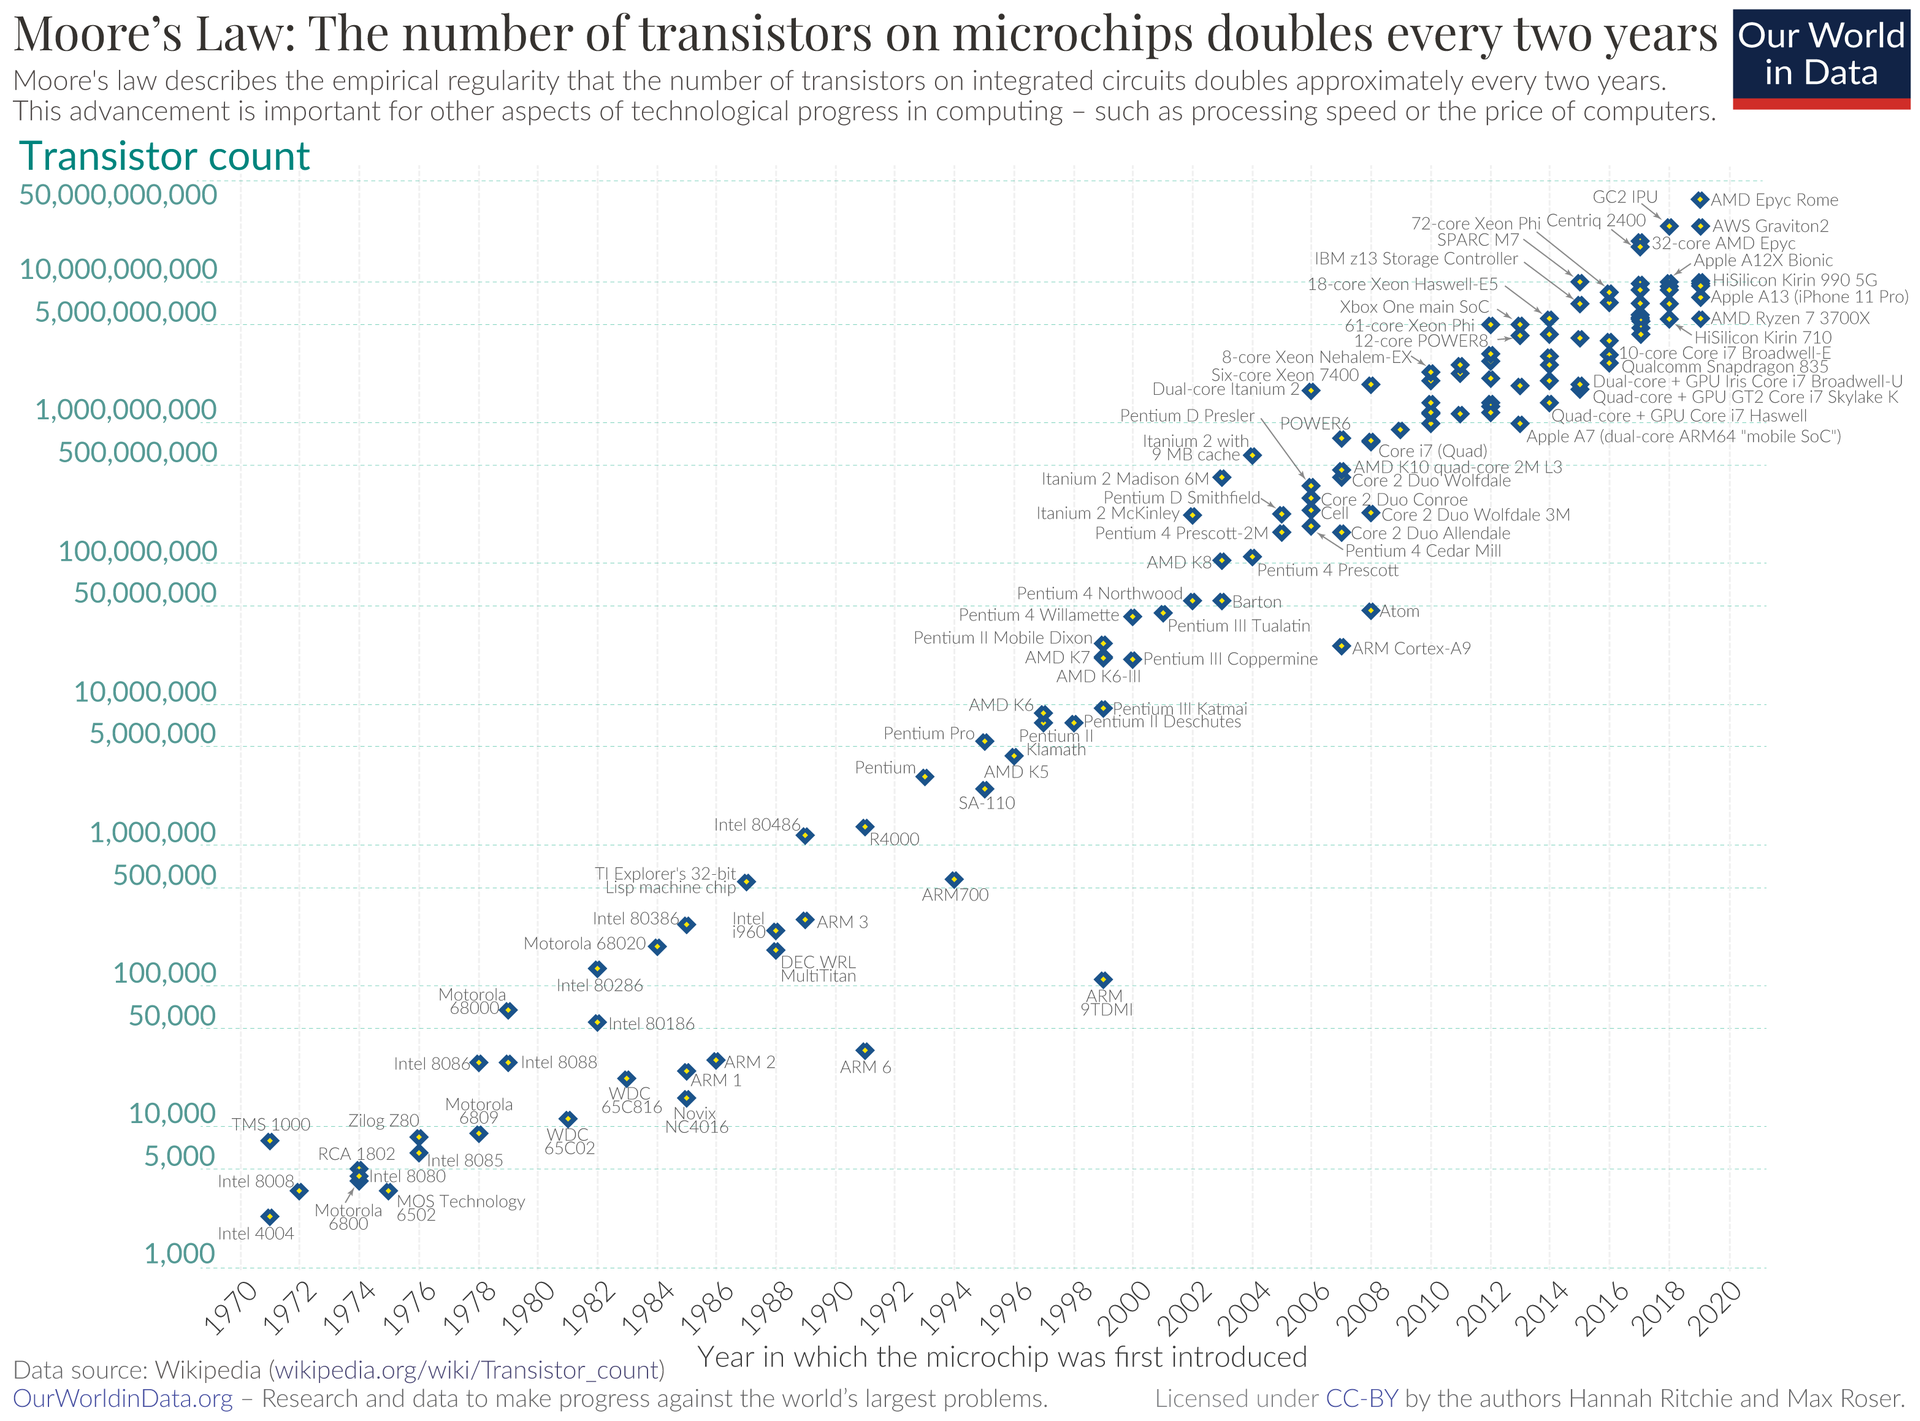
\includegraphics[width=1\linewidth]{img/rationalchoice/moore} 

}

\caption{Moores Law}\label{fig:rationalchoice1}
\end{figure}

\hypertarget{marginal-costs-and-benefits}{%
\section{Marginal Costs and Benefits}\label{marginal-costs-and-benefits}}

We will now illustrate the foundations for a model of rational choice. Whenever we make a choice we weigh, if we are rational, the costs of the action and the benefits of the action. We will start with an action that can be chosen in small increments.

Examples of such actions are:

\begin{itemize}
\tightlist
\item
  How many miles do I want to hike this coming weekend?
\item
  How much money do I want to contribute to a charity?
\item
  How much time do I want to spend texting my parents while I'm getting ready for my exam in college?
\item
  How much time do I want to study for the final in my introductory economics course?
\item
  How much chocolate do I want to eat this week?
\end{itemize}

In all of these cases, the choice is a continuous variable, the choice is not a discrete, all or nothing kind of choice.

Of course, there are many choices that are of the all-or-nothing variety:

\begin{itemize}
\tightlist
\item
  Getting on an airplane to fly to San Diego during covid-19: yes or no?
\item
  Attending IU: yes or no?
\item
  Marrying my high-school sweetheart: yes or no?
\end{itemize}

In a sense the all or nothing choices are relatively easy to model and understand. If you think you are better off marrying your high-school sweetheart than not, in econ speak, if the benefit of marrying your high-school sweetheart exceeds the cost, whatever you think that might be, and we have to come back to that, then by all means the decision should be: marry your high school sweetheart. (Of course, it takes two to tango.)

The decisions where continuous choices are involved might be somewhat harder to model. This is what we are embarking on now. We need some terminology.

The marginal benefit of an action, MB, is the extra benefit obtained by carrying out the action one more unit.

The marginal benefit of hiking one extra mile is the enjoyment I get out of being in nature for another 20 to 30 minutes or so. And, of course, it is the extra calories I burn by hiking one extra mile so I can eat more cookies when I get home.

The marginal benefit of studying for the exam in my economics class is the extra understanding of the material I gain, and it includes the increased probability that I ace the exam.

The marginal benefit of talking to my mom on the phone for an extra half-hour is simply the enjoyment of communicating with my mom and it could include some extra probability of getting my allowance increased.

The marginal cost of an action, MC, is the extra cost incurred by carrying out the action one more unit.

The marginal cost of hiking one extra mile includes a bunch of things. In that extra time, 20 or 30 minutes, I could be doing all kinds of other things, like sitting on my back porch and eating cookies. If I hiked an extra mile, I might get so tired that I lose concentration, stumble over a rock or a root, fall and break an ankle. If I hiked an extra mile, I run an extra risk of getting lost and I might not be able to get back home on time for an important appointment.

The marginal cost of studying an extra hour for the exam in my economics class includes not studying for the exam in my chemistry class and it includes things like watching TV or hanging out with my friends.

The marginal cost of communicating with my mom on the phone includes not studying for my economics exam.

You get the idea. If I commit sometime to one particular action, there are a whole bunch of other things I cannot do at the same time. If I donate \$100 to one charity, I cannot donate it to another charity. If Jose works in industry 1, he cannot work in industry 2.

This brings us to the notion of opportunity cost.

Opportunity cost is one of the most important concepts in economics, if not the single most important one and it is crucial that we have a firm grasp off this concept.

The definition of opportunity cost is simply: the value of the next best alternative forgone by making a particular choice.

Let's consider the following possibilities ranked in order pleasure or utility I derive from them:

\begin{enumerate}
\def\labelenumi{\arabic{enumi}.}
\tightlist
\item
  reading a good book
\item
  reading the New York Times
\item
  reading a letter from my son
\item
  going for a walk
\item
  talking to my brother on the phone
\item
  cleaning the gutters on my roof
\end{enumerate}

And there are many others. If these are really listed in order of priority and importance for me, I will choose reading a good book.

What is the opportunity cost of reading a good book? It is not the pleasure I get out of talking to my brother on the phone. That is the fifth best thing I could be doing at that moment. The opportunity cost of reading a good book is reading the New York Times. Reading the New York Times is my next best alternative after reading a good book. So, the opportunity cost of reading a book is the value I would have derived from reading the New York Times, my second-best alternative forgone.

\hypertarget{choice}{%
\section{Choice}\label{choice}}

We will now present our basic and simple model/theory of rational choice. We make two assumptions.

\begin{center}
\textbf{Assumption 1: The marginal benefit of an action, MB, is declining as the action is increased.}

\end{center}

When we graph the marginal benefit of an action it will be downward sloping. In Economics this assumption is known as

\begin{center}
Diminishing returns (or diminishing utility)

\end{center}

This is an assumption, not a universal law, that makes sense in many situations, not in all. We will address some exception later on. But in many situations, this makes sense.

After cutting grass in my backyard on hot Saturday in July, the first sip or glass of sweetened iced tea just tastes great and quenches my thirst. The second glass a little bit less, the fourth glass not so much.

That first hour of a hike on a mild fall day feels wonderful. By the third hour I feel tired and my back hurts from carrying a backpack.

Seeing a boyfriend/girlfriend for the first time after a long separation can feel like heaven. After a few days/weeks, the routine has set in, the elation and excitement are gone.

A few years ago, there was a solar eclipse that could be seen mid-afternoon, with the proper protective glasses of course. I remember feeling very excited about stepping out of my building on the way to class with my protective gear. Seeing the eclipse was stunning, truly stunning. I just kept looking and looking. But after three or so minutes, the excitement had warm off. Diminishing returns had set in in my case. Evidently, something very similar had happened to most of the IU students I saw along the way. The administration had made allowances for the students to be out of class so they could watch the eclipse. Huge numbers of students were outside. They were outside, but were they enthralled by the eclipse? Evidently not. Most of them were just chatting with each other, ignoring the eclipse. Their diminishing returns had set in even before mine.

Pricing for Disney theme parks in Florida also displays an example of diminishing returns; in this case the diminishing returns refer to the pleasure Mickey Mouse fans may experience from visiting the Magic Kingdom. On the Disney website you can purchase tickets for visits between 1 and 10 days. Wow, 10 days in the Magic Kingdom! What magic!

Here are the total prices for tickets for 1 to 10 days, at least as of 08/18/21.

\begin{longtable}[]{@{}ccc@{}}
\toprule
\# of Days & Total Price & Difference per Day \\
\midrule
\endhead
1 & 109 & 105 \\
2 & 214 & 101 \\
3 & 315 & 97 \\
4 & 412 & 28 \\
5 & 440 & 10 \\
6 & 450 & 19 \\
7 & 469 & 19 \\
8 & 488 & 16 \\
9 & 504 & 16 \\
10 & 520 & 16 \\
\bottomrule
\end{longtable}

Evidently there is a large drop after day 4. Why? If the marginal benefit of the ninth day were as high as the marginal benefit of the second day, surely Disney would change its pricing scheme.

\begin{center}
\textbf{Assumption 2: The marginal cost of an action, MC, is increasing as the action is increased.}

\end{center}

The graph of marginal cost is upward sloping.

This also goes by the name of diminishing returns.

This is also an assumption, not a universal law. In many cases this assumption rings true.

Imagine studying for a chemistry exam the night before the exam. You have not really kept up well with the material in that class and you know you will have to study way past midnight to have a shot at doing well. You start studying right after dinner at 7 pm. The mental effort required to learn is higher at midnight than at 10 pm and at 10 pm it is higher than at 8 pm. Your consumption of coffee or power drinks goes up as time goes on.

Studying each chapter gets harder and harder the longer you study. The effort required to understand a given chunk of material goes up over time. The marginal cost of acquiring knowledge rises. That is diminishing returns.

We can now put together the marginal benefit of an action and the marginal cost of the action. This is done in Figure 2. Let a, on the horizontal axis, denote the extent of the action. MB and MC of that action are graphed on the vertical axis. For the sake of concreteness, assume we are talking about how long Leslie should study for her chemistry exam.

\begin{figure}

{\centering 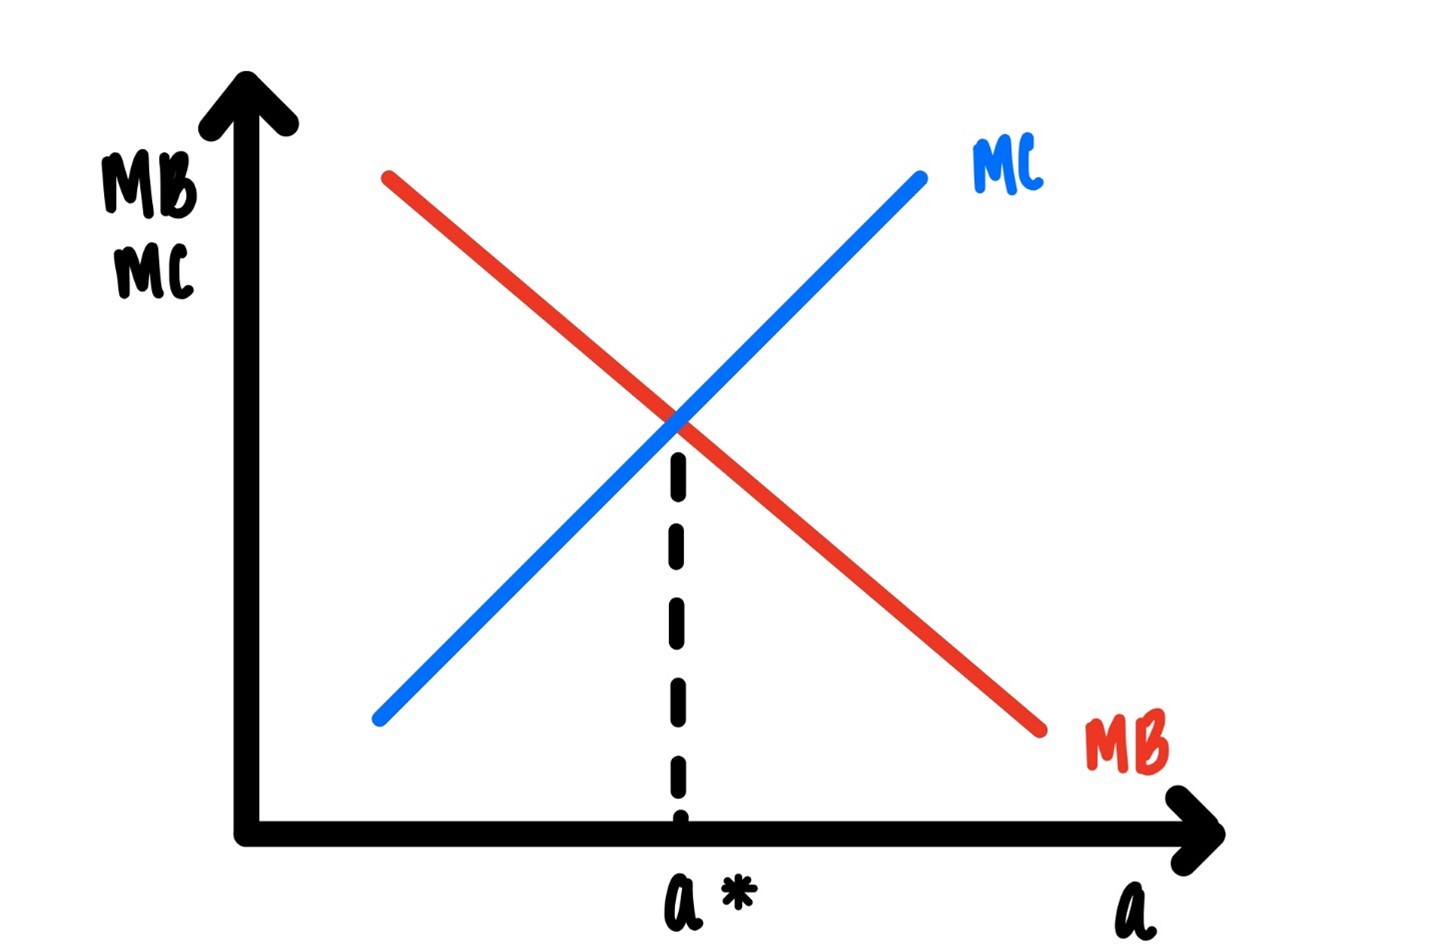
\includegraphics[width=0.75\linewidth]{img/rationalchoice/fig2} 

}

\caption{Rational Choice,}\label{fig:rationalchoice02}
\end{figure}

In Figure \ref{fig:rationalchoice02}, the marginal benefit of the action, MB, is downward sloping in accordance with assumption 1. The marginal cost of the action, MC, is upward sloping in accordance with assumption 2.

Claim: The optimal amount of time Leslie should study for the chemistry exam, IF Leslie is rational, is given by a*.

Why? Imagine that Leslie did anything else. Imagine she studied less, only a1. At that point, the marginal benefit of studying an extra half hour exceeds the marginal cost. So, Leslie should study an extra half hour. She should study more. She should move from a1 to the right closer to a* as indicated by the arrow pointing right. If Leslie is rational, she will do just that.

Imagine Leslie studies more, say a2. At that point, the marginal cost of studying that last half hour exceeds the marginal benefit. Sleep deprivation does not usually translate in high exam scores. At a2 Leslie should decide to study less. She should move to the left, as indicated by the arrow pointing left. Rational Leslie will do just that.

We have established in the case of Leslie studying for her exam, but much more generally:

\begin{iucolor}
\textbf{Rational action requires that the marginal benefit of an action is equated to the marginal cost of an action.}

\end{iucolor}

This conclusion which is illustrated in Figure \ref{fig:rationalchoice02} above will provide the basis for about 80\% of the material in this class. Figure 2 will show up in this class, again and again, just in different contexts.

In Figure \ref{fig:rationalchoice02}, the marginal benefit curve is downward sloping, and the marginal cost is upward sloping. We will encounter three versions of Figure \ref{fig:rationalchoice02} in this course. They are just very slight variations of Figure \ref{fig:rationalchoice02}. These are depicted in Figure \ref{fig:rationalchoice03}. Panel a is just a reproduction of Figure \ref{fig:rationalchoice02}. In panel b, the marginal benefit curve is a horizontal line, and the marginal cost is upward sloping. In panel c, the marginal benefit is downward sloping, and the marginal cost is a horizontal line.

\begin{figure}

{\centering 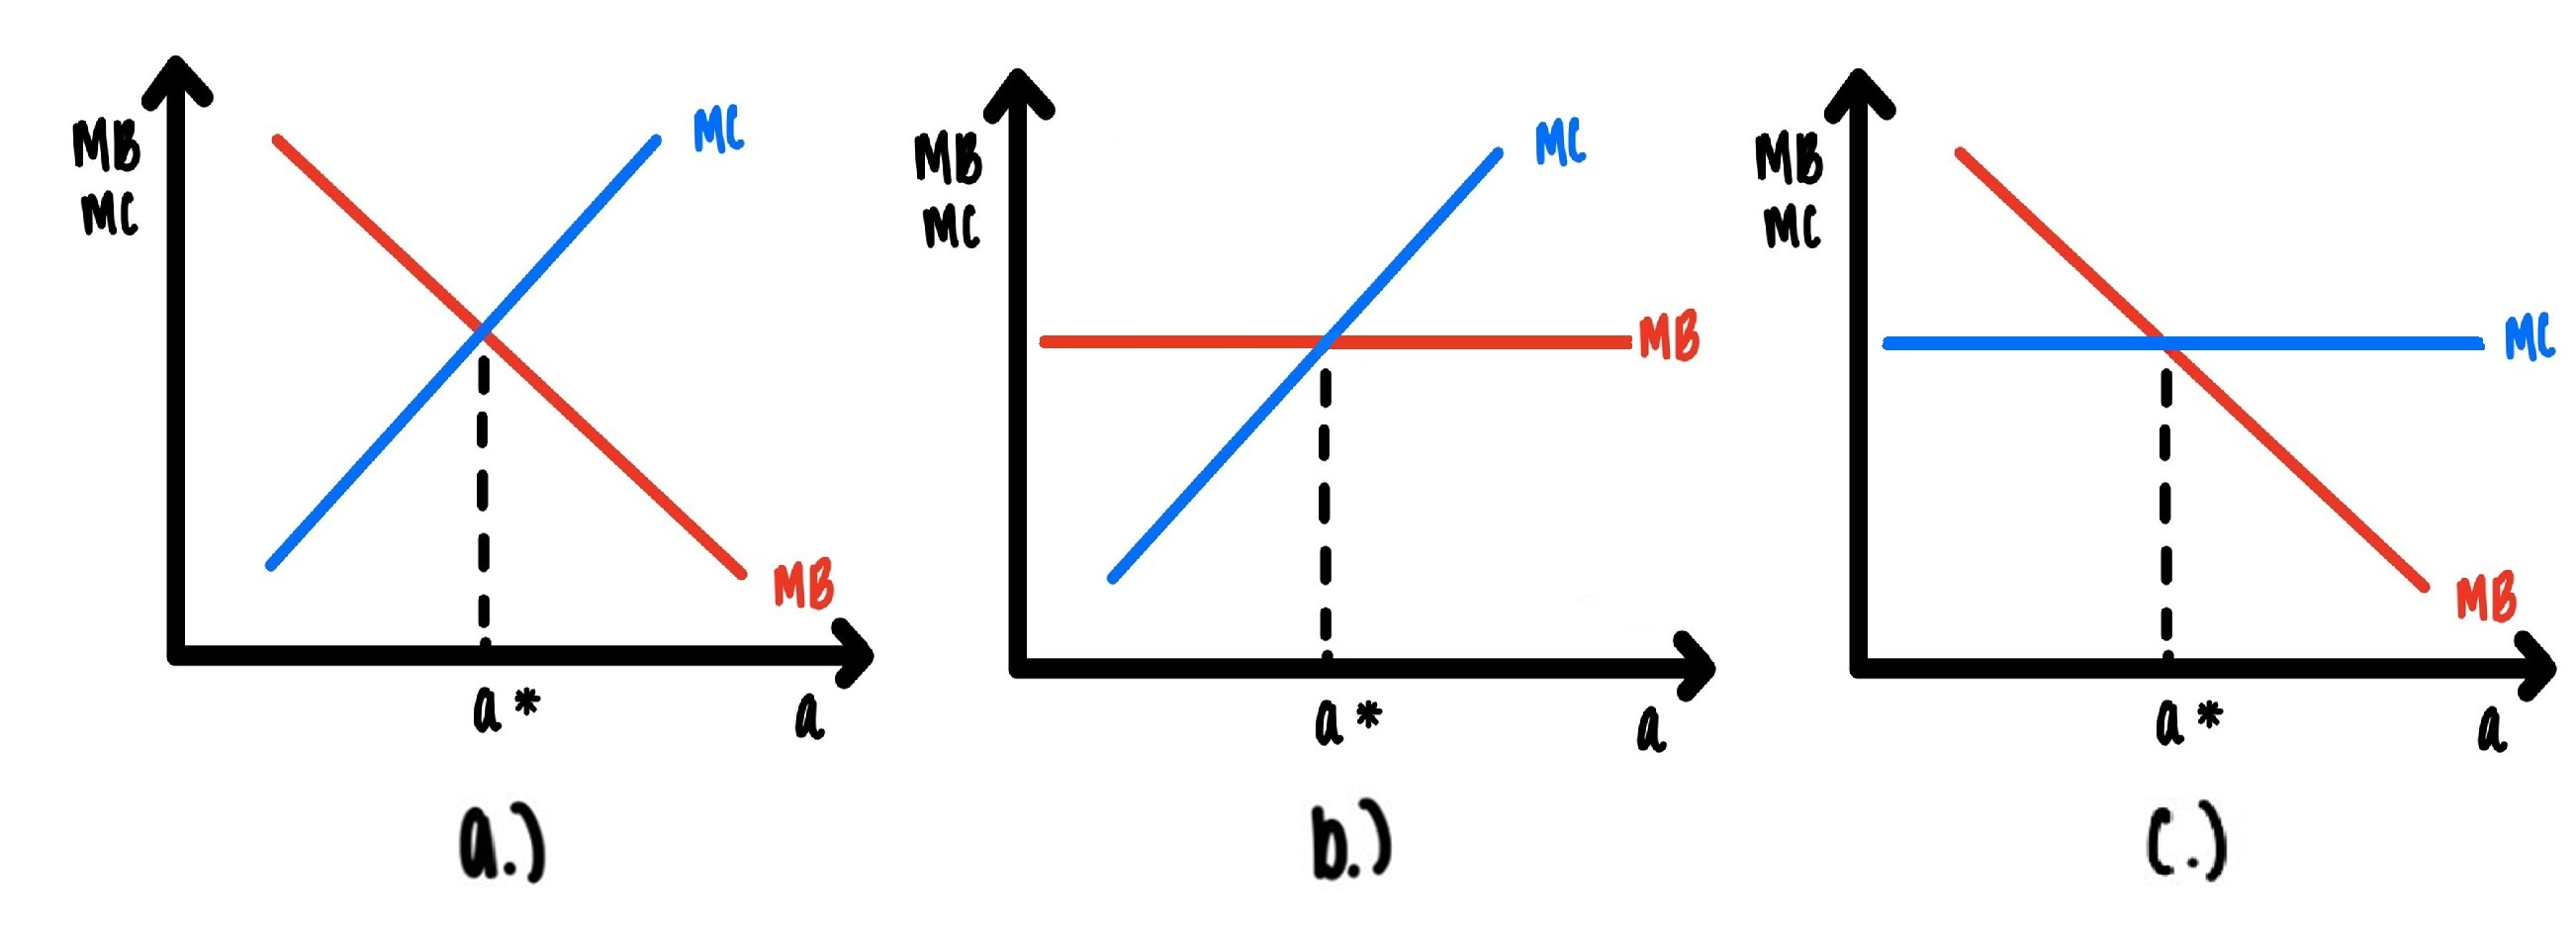
\includegraphics[width=1\linewidth]{img/rationalchoice/panels} 

}

\caption{This photo will reappear many times!}\label{fig:rationalchoice03}
\end{figure}

We can get from panel a to panel b by rotating the marginal benefit curve downward, so it becomes horizontal. We can get from panel a to panel c by rotating the marginal cost downward, so it becomes horizontal.

While these panels look slightly differently, they are just slightly different versions of the same thing:

At low levels of the activity, marginal benefit is above marginal cost. At high levels of the activity, marginal cost is above the marginal benefit. Somewhere in between there is a sweet spot, where marginal benefit equals marginal cost.

\hypertarget{shifting-curves}{%
\section{Shifting Curves}\label{shifting-curves}}

What if some event occurs in which the marginal benefit or cost of an action changes?

The environment in which we live is not static. Our circumstances change all the time. In the framework laid out above there will be frequent changes in the marginal benefits and the marginal costs for our actions. How do these shifts influence rational action?

In Figure \ref{fig:rationalchoice04} we show how an increase in the marginal benefit of the action changes our rational choice.

\begin{figure}

{\centering 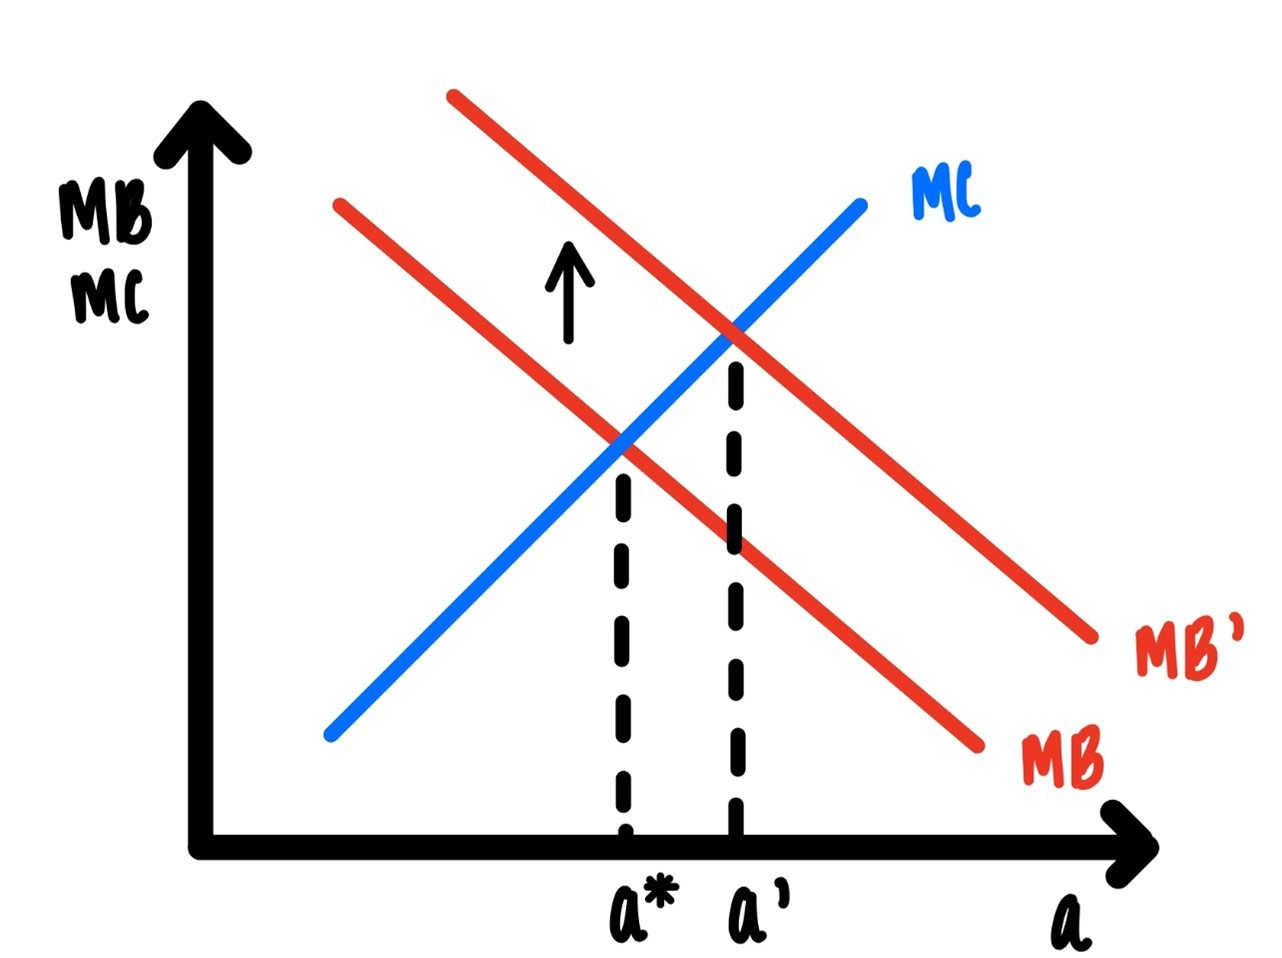
\includegraphics[width=0.75\linewidth]{img/rationalchoice/fig4} 

}

\caption{Increase of Marginal Benefit}\label{fig:rationalchoice04}
\end{figure}

Imagine that you are planning on a 3-hour hike by yourself this coming Saturday. Saturday morning your best friend calls you up and tells you he has nothing to do that day. You are overjoyed and invite him on the hike. Hiking with your best friend is much more enjoyable than a solitary hike. Because your friend accompanies you on your hike, the marginal benefit curve shifts out (Figure \ref{fig:rationalchoice04}) to the right. As a consequence, your 3-hour hike turns into a 4-hour hike. That is the rational response.

In Figure \ref{fig:rationalchoice05} we show how an increase in marginal cost of the action changes your rational choice.

\begin{figure}

{\centering 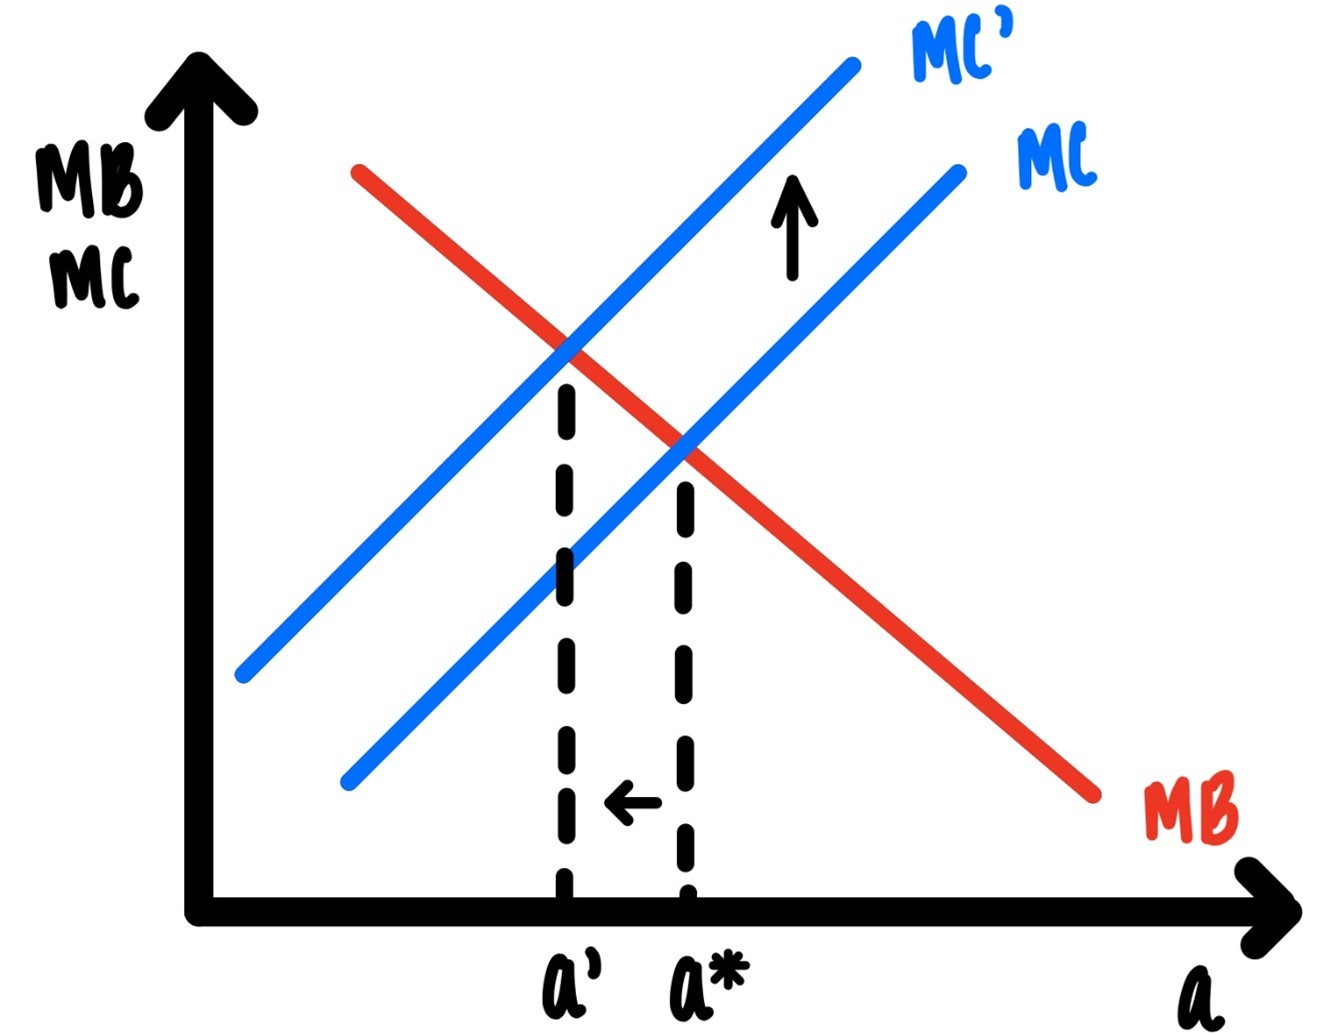
\includegraphics[width=0.75\linewidth]{img/rationalchoice/fig5} 

}

\caption{Increase of Marginal Cost}\label{fig:rationalchoice05}
\end{figure}

Imagine you are planning a 3-hour hike for this coming Saturday. Saturday morning your wake up and you realize that overnight there was torrential rain that turned the hiking trails in your area into mud. Each step is a muddy slog. Each step now is drudgery. The rain has increased the marginal cost of hiking (Figure \ref{fig:rationalchoice05}). Your 3-hour hike turns into a 2-hour hike. That is the rational response.

\hypertarget{examples-of-rational-choice}{%
\section{Examples of Rational Choice}\label{examples-of-rational-choice}}

\textbf{(Refreshing Lemonade)} You just cut the grass on a hot July afternoon. You are hot, sweaty, parched. Figure \ref{fig:rationalchoice06} captures the marginal benefit and the marginal cost of drinking lemonade. Assume the units of measurement are small glasses. The marginal cost of drinking lemonade is just the cost of each glass of lemonade. It is the same for each small glass. It is a horizontal line. The marginal benefit declines with each glass. The first glass is a great thirst quencher and so is, perhaps the second glass. Glasses three and four less so. By the sixth glass the marginal benefit is tiny, below marginal cost. It is rational for you to drink 4 glasses.

\begin{figure}

{\centering 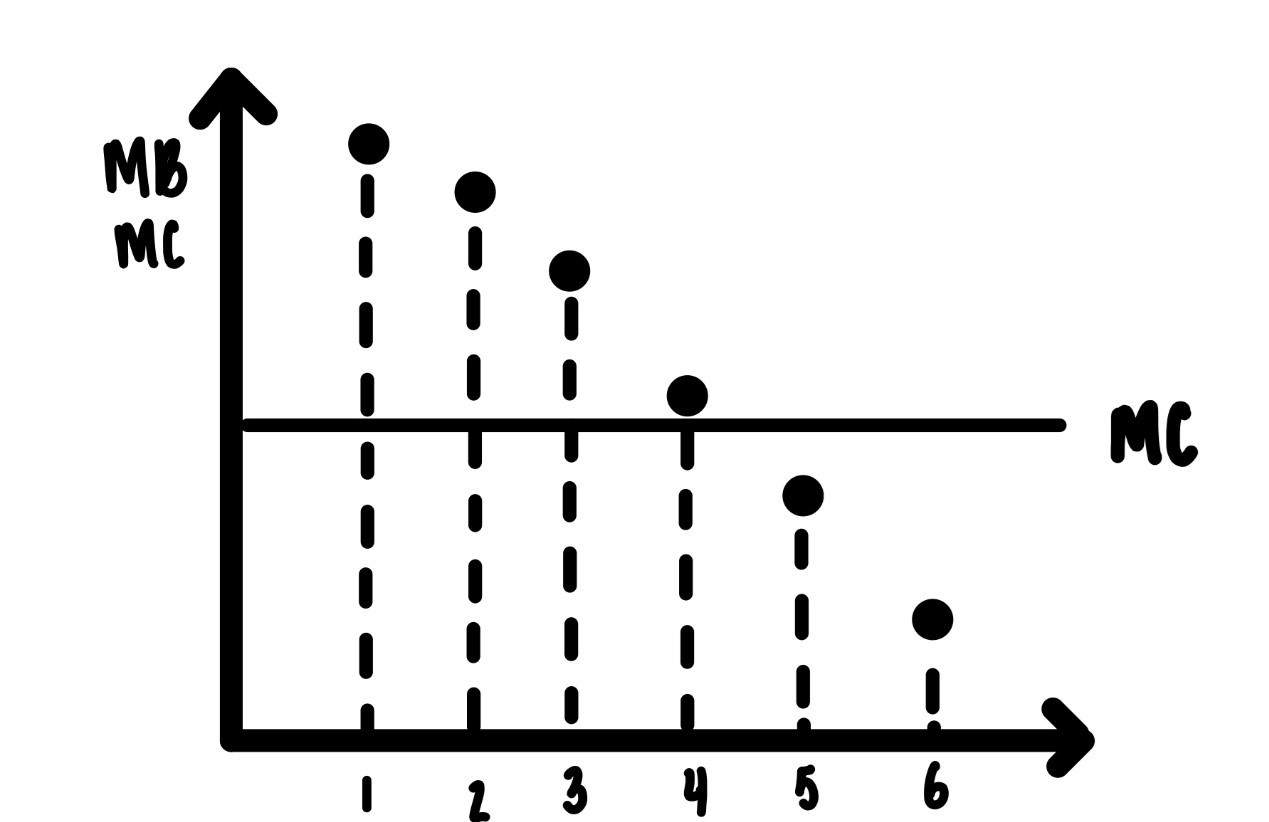
\includegraphics[width=0.5\linewidth]{img/rationalchoice/fig6} 

}

\caption{Drinking lemonade on a hot Saturday afternoon after you cut the grass.}\label{fig:rationalchoice06}
\end{figure}

\begin{center}\rule{0.5\linewidth}{0.5pt}\end{center}

\textbf{(Optimal Retirement)} Joe is dedicated high school math teacher. He has been teaching for 38 years and he has been planning to teach until his 70th birthday. That was his optimal choice, after careful consideration of the joys of teaching, the marginal benefit in econ speak and the costs. He has noticed that in the last few years it has become harder to get up with a spring in his step every morning, it has become harder to concentrate while grading papers. Yet, he still likes his job, with the joys outweighing any negative considerations. Then Covid-19 hit. Online teaching, lack of resources, concern for his health, administrative back and forth, administrative indecision, opinionated parents who seem to stand in the way of effective teaching. His marginal benefit has shifted way down. Now, retirement at age 65 instead of age 70 looks very appealing, and rational. \href{https://www.npr.org/2020/11/18/936096303/nurses-are-under-pressure-as-hospitals-strain-to-meet-pandemic-demands}{It appears, nurses are in the same storm.}

\begin{figure}

{\centering 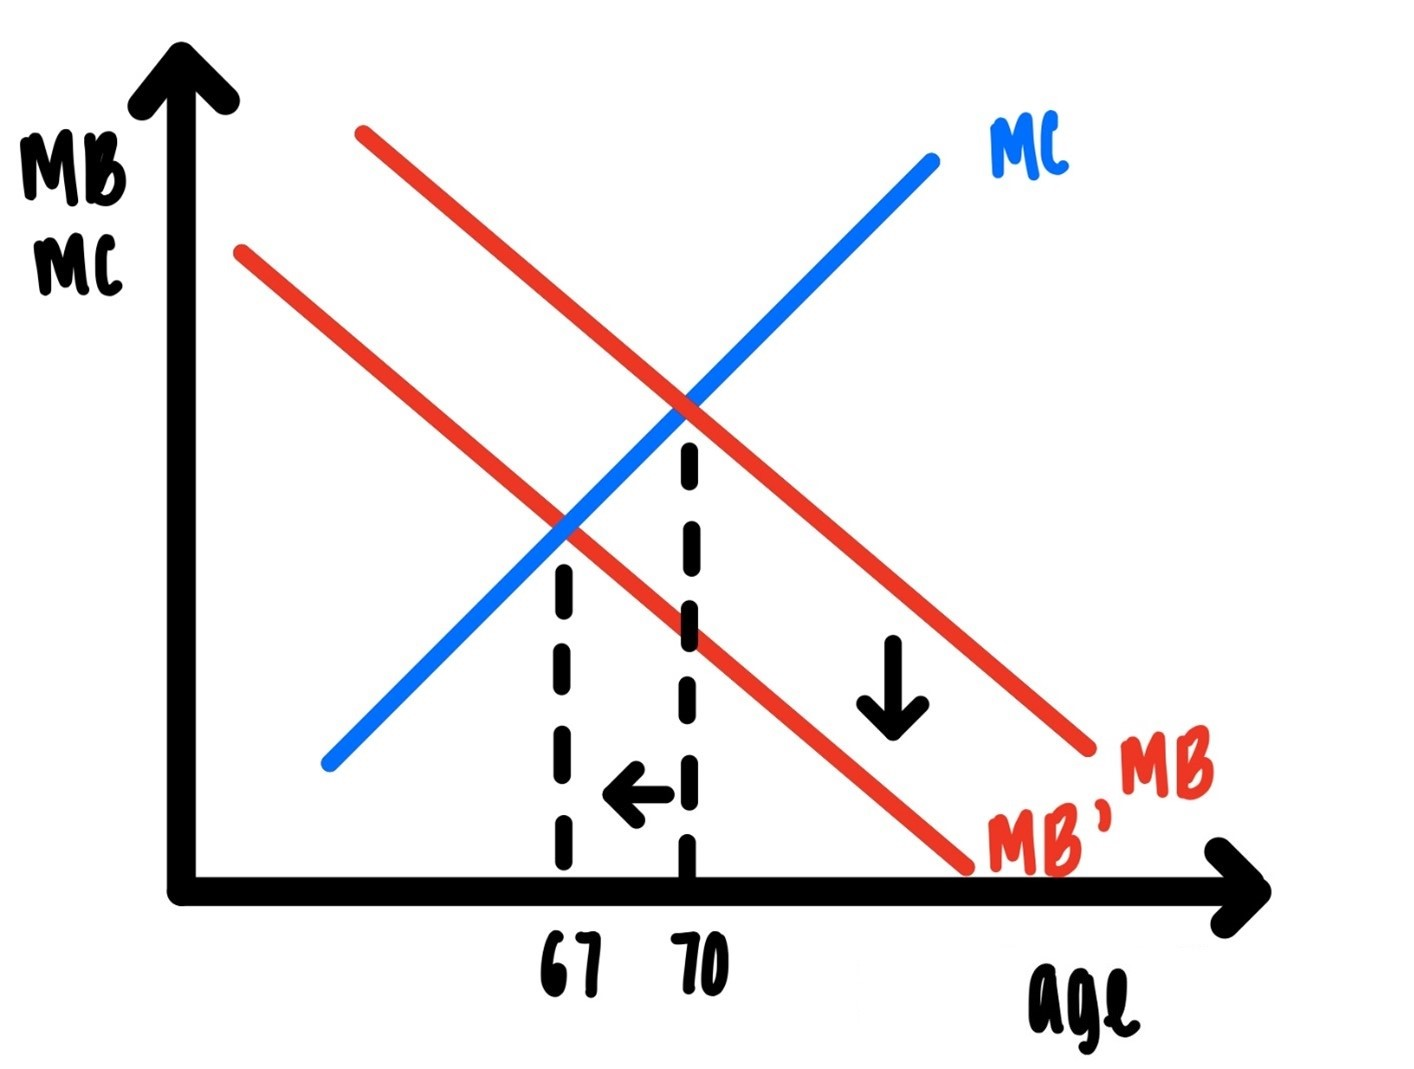
\includegraphics[width=0.75\linewidth]{img/rationalchoice/fig7} 

}

\caption{Optimal retiring age.}\label{fig:rationalchoice07}
\end{figure}

\begin{center}\rule{0.5\linewidth}{0.5pt}\end{center}

\textbf{(Optimal Family Size)} What is our optimal number of kids? I know the number of children is not a continuous variable like how long to hike or how long to study for an exam. We still can imagine that there is a marginal benefit from having children and a marginal cost. Let's assume for the sake of simplicity that the marginal cost of a child is constant. I know that things like hand me down clothes might make the second child cheaper than the first, but this will not matter for the argument here. I also know that some parents look forward to having several children, rather than just one to see their children play with each other and grow up with each other. One could make therefore an argument that the marginal benefit of the second child might be higher than the marginal benefit from child number 1. Again, this would not influence the argument here. The point is that eventually the marginal cost of an extra child is higher than the marginal benefit of that child.
One interesting fact about desired fertility in the US seems to be: Whatever the number of children, if there is no boy among these children, the probability of having another child goes up. Suppose that for child 3, the marginal benefit is just above the marginal cost. Then the optimal rational number of children is 3. But things don't stop here. The sex composition of children seems to matter for the decision to have another child. If all three previous children are girls, indicated by the string (G, G, G), then the marginal benefit of having a fourth child is high, above marginal cost and the family has a fourth child. If there is at least one boy among the first three, indicated by the potential strings (B, G, G), (G, B, G), (G, G, B), (B,B, G), (G, B, B), then the marginal benefit of a fourth child is low. The family will only have three children.
That's the theory. That is also in the data. \url{https://econweb.ucsd.edu/~gdahl/papers/demand-for-sons.pdf}\\
American families tend to have a preference for sons over daughters.

\begin{figure}

{\centering 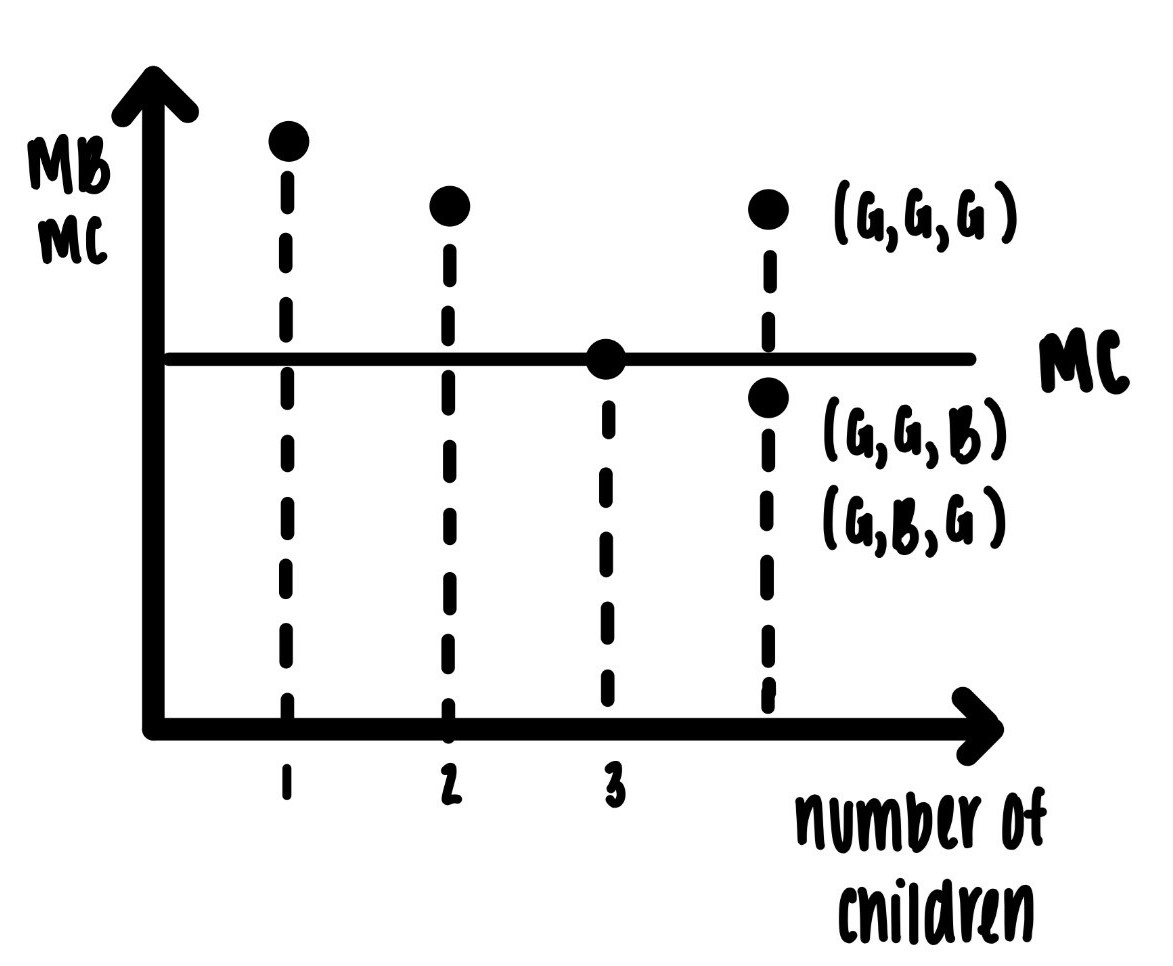
\includegraphics[width=0.5\linewidth]{img/rationalchoice/fig8} 

}

\caption{Optimal fertility}\label{fig:rationalchoice08}
\end{figure}

\hypertarget{increasing-returns}{%
\section{Increasing Returns}\label{increasing-returns}}

We said earlier that diminishing returns is not an iron law. It is an assumption that is helpful in many cases. We have seen some examples above. There are cases where there are not diminishing but increasing returns.

Suppose you want to build a bridge over the Mississippi just north of St.~Louis. It will require a ton of concrete. The point of the bridge is to get more transportation services from IL to MO and back. The marginal cost of the concrete can be assumed to be constant as seen in Figure \ref{fig:rationalchoice09}.

\begin{figure}

{\centering 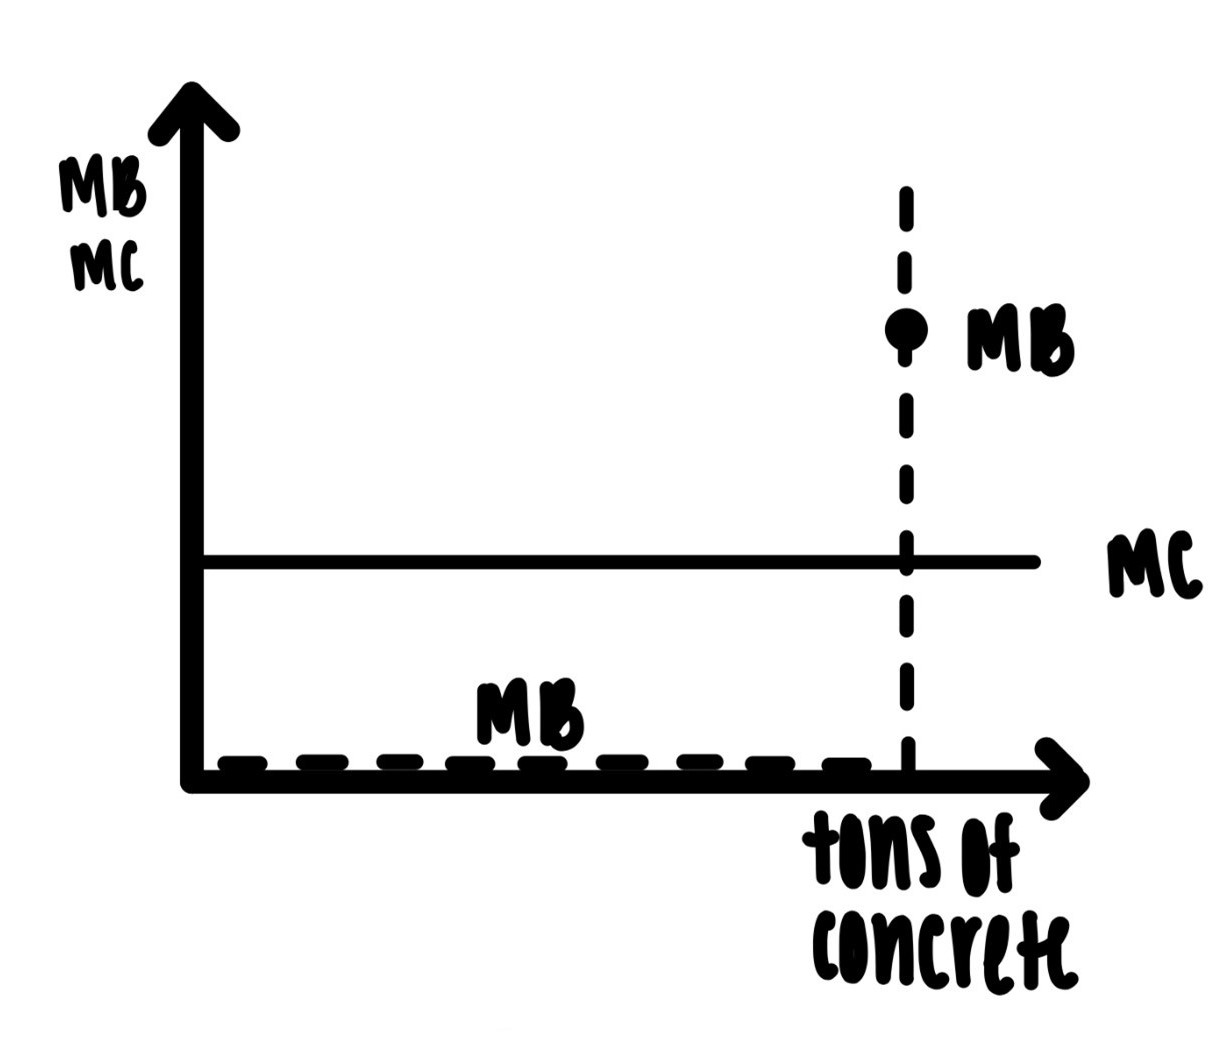
\includegraphics[width=0.75\linewidth]{img/rationalchoice/fig9} 

}

\caption{Concrete for bridge}\label{fig:rationalchoice09}
\end{figure}

The marginal benefit derived from the concrete is the shape of an inverted L. It is basically zero for practically every ton of concrete. There will be no transportation services at all until the very last ton of concrete is used to complete the bridge. Only when the last ton of concrete is laid, will there be any transportation services. Hence the inverted L shape.

\begin{center}\rule{0.5\linewidth}{0.5pt}\end{center}

Suppose a widow, mother of two young children is \(\$750\) behind on utilities. If she cannot pay the utility bill by next week, the power company will disconnect her service. Apart from not being able to heat the apartment and cook, disconnect from the power company means loss of her Section 8 housing and she and her two children will be homeless. Joe is a generous soul and gives her \(\$200\). That helps just a little bit, but her utility will still be shut off and she still faces the prospect of homelessness with her kids. Generous Jill pitches in another \(\$200\), and so does generous Jacqui. The marginal benefit of each one of these contributions is relatively small, since even with \(\$600\) she still faces the prospect of homelessness. Generous Jack finally pitches in another \(\$200\). This helps her over the top. It might be reasonable to assume that the marginal benefit to the widow of these contributions is as indicated in Figure \ref{fig:rationalchoice10}, convex at first, below the \$750 threshold and concave on the other side.

\begin{figure}

{\centering 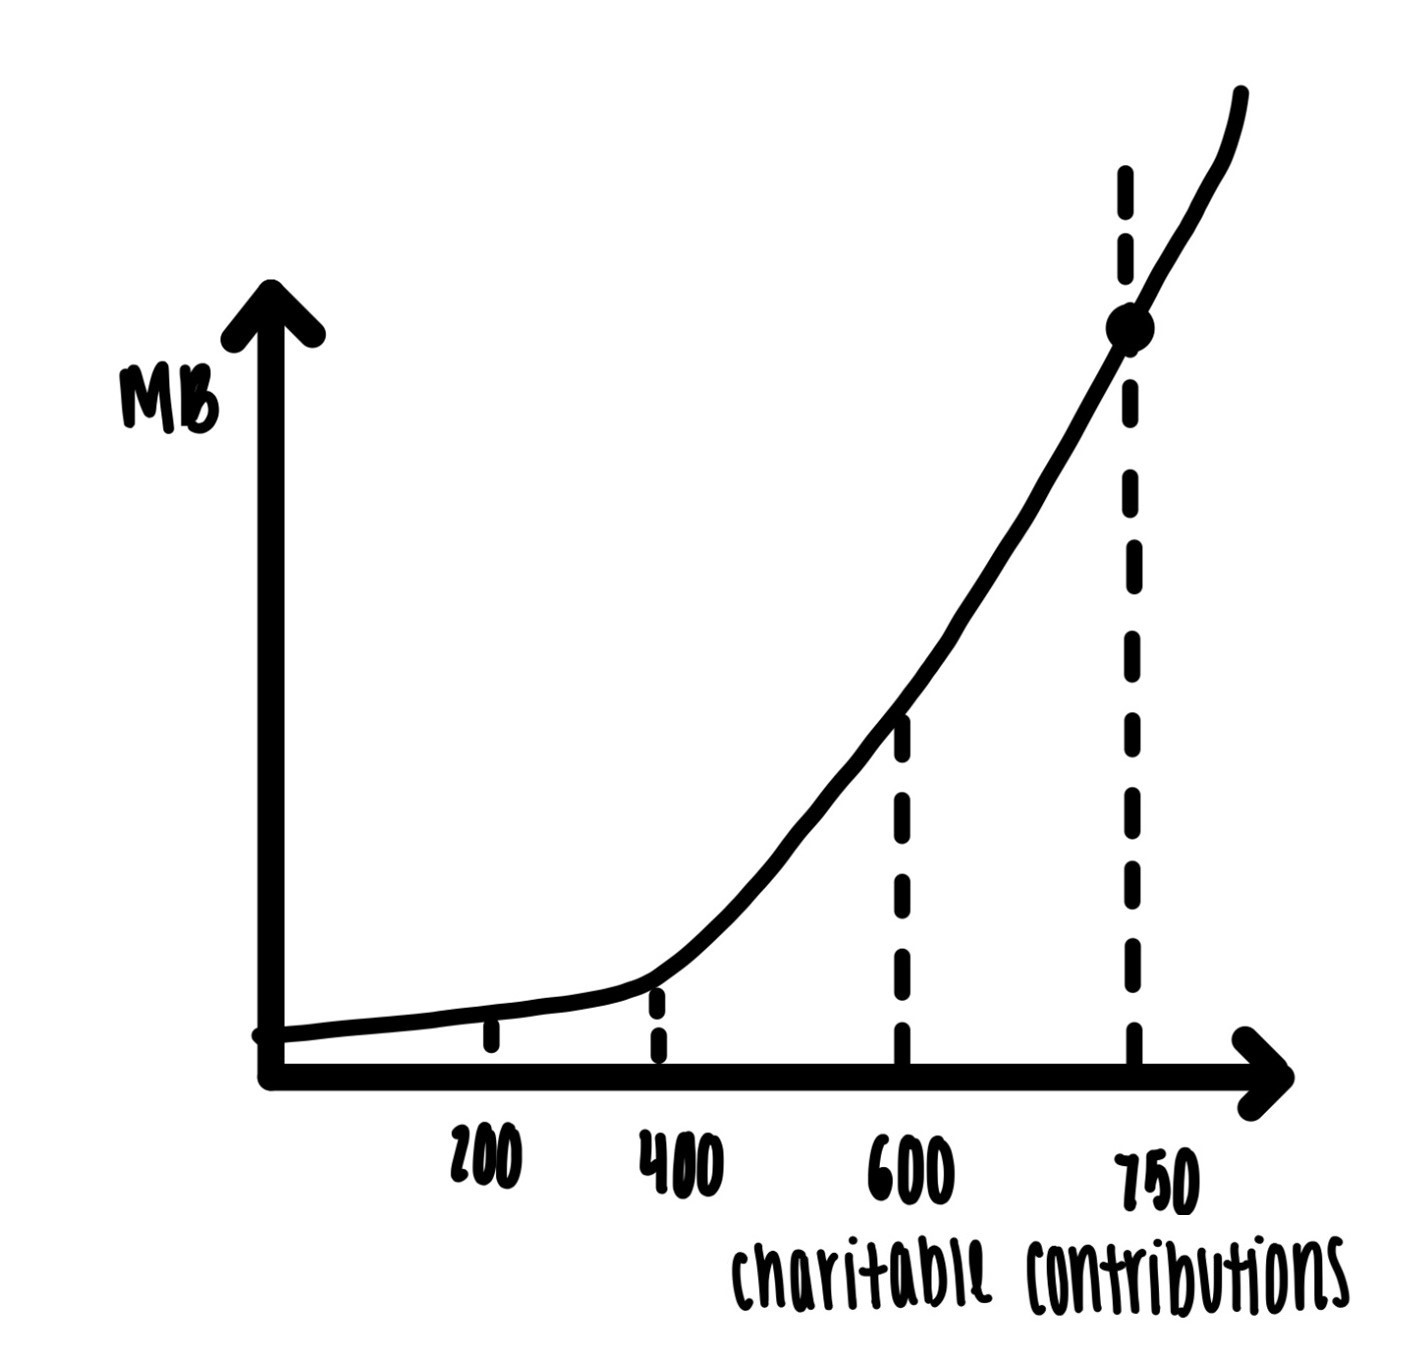
\includegraphics[width=0.75\linewidth]{img/rationalchoice/fig10} 

}

\caption{Benefit to widow of charitable contributions}\label{fig:rationalchoice10}
\end{figure}

\begin{center}\rule{0.5\linewidth}{0.5pt}\end{center}

Why do you go to school? When I ask students that question the answer is invariably: To get a better job. And when I ask: What is a better job? the answer very often is something like: More money. The connection between schooling, years of schooling, and wages or earnings is one of the age-old central topics in labor economics.\footnote{\url{https://en.wikipedia.org/wiki/Mincer_earnings_function}}

\begin{figure}

{\centering 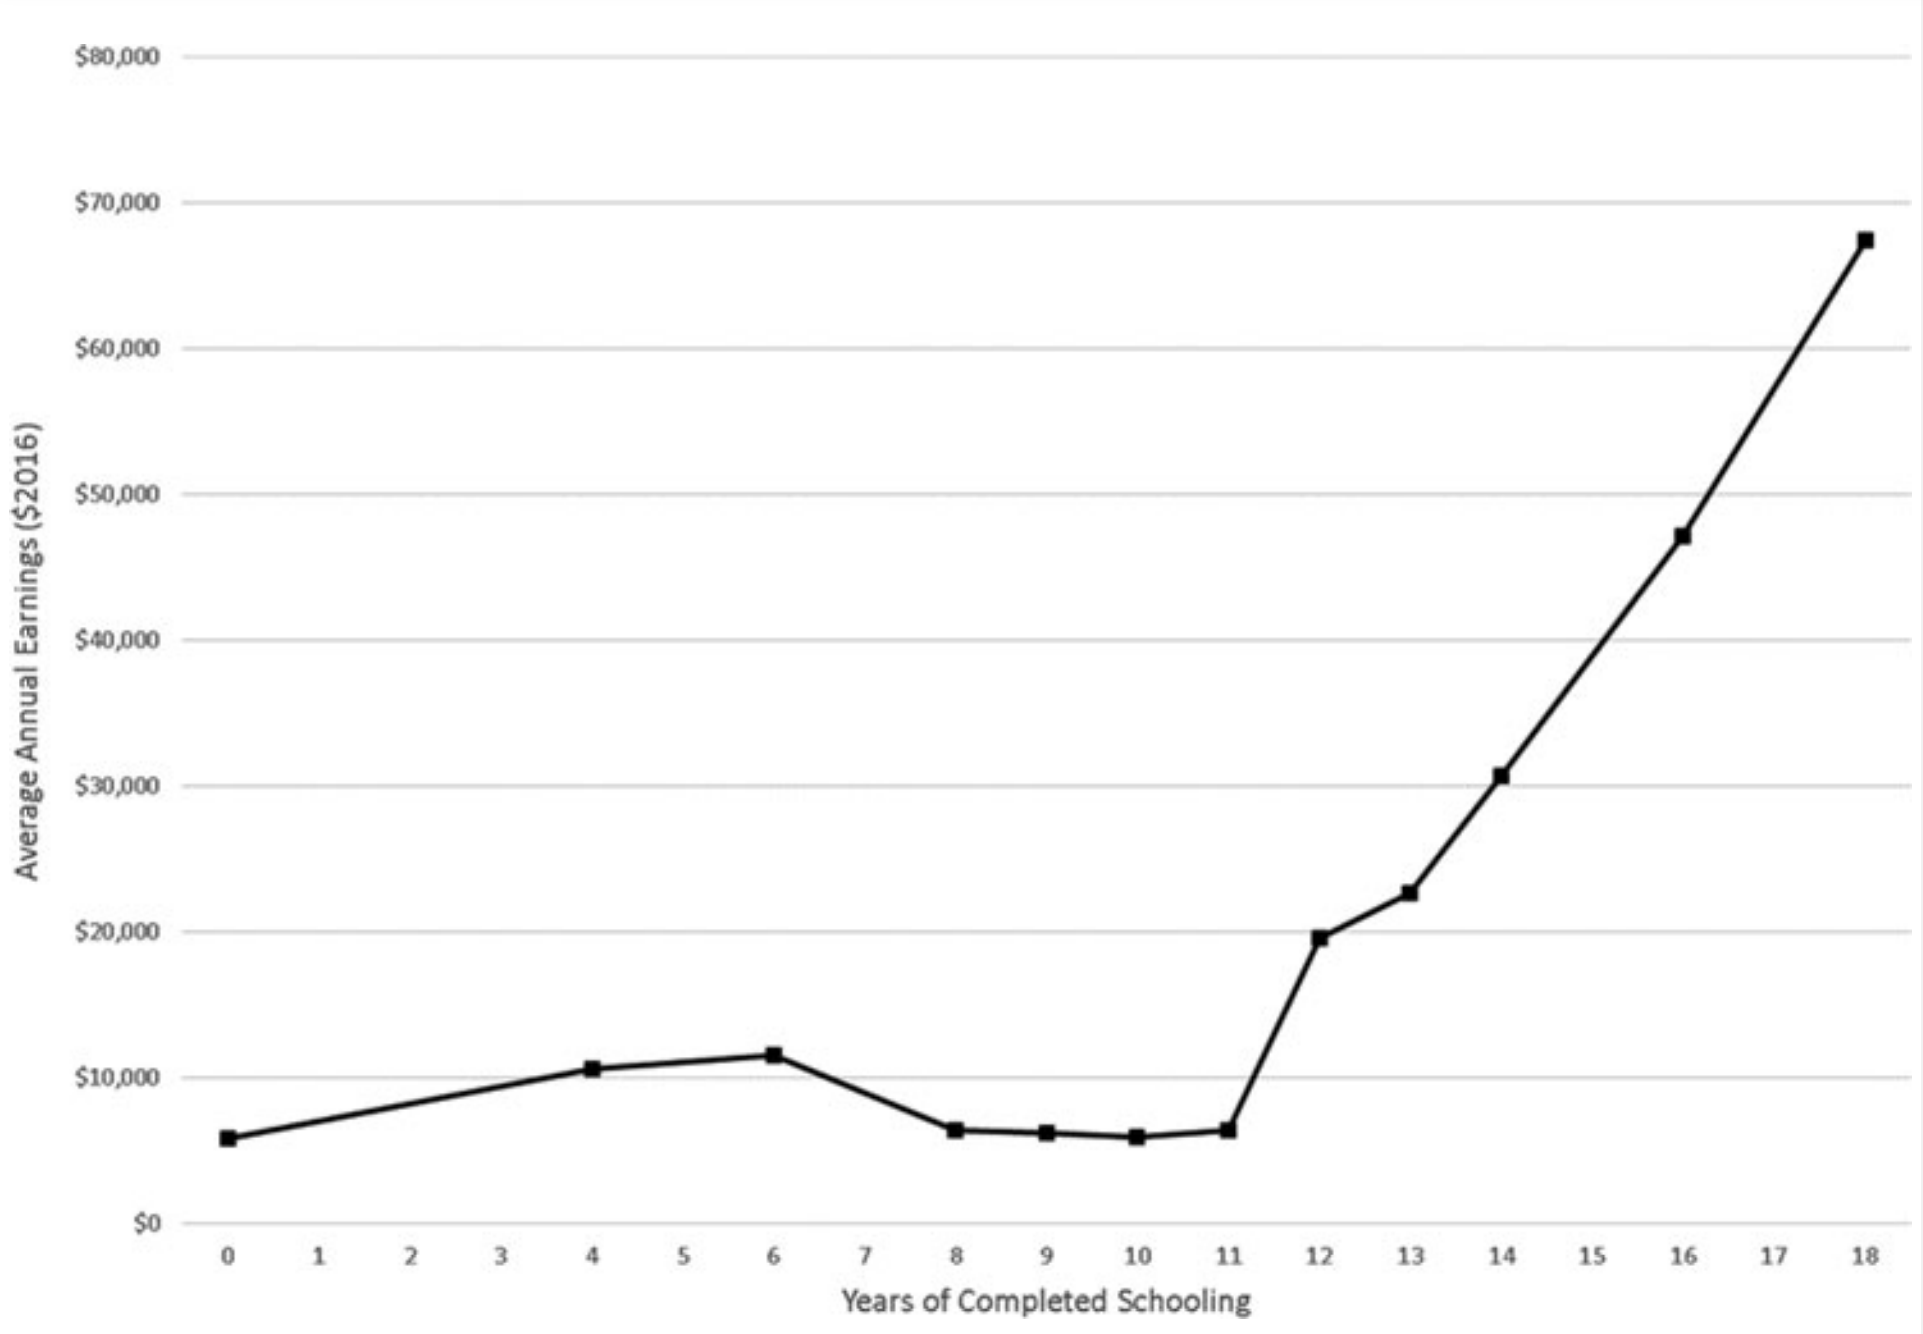
\includegraphics[width=1\linewidth]{img/rationalchoice/fig11} 

}

\caption{Source: Cecilia Elena Rouse, 2017, The economics of education and policy: Ideas for a principles course, The Journal of Economic education, 48:3, 229-237}\label{fig:rationalchoice11}
\end{figure}

The return to an extra year of schooling is basically zero between 1 and 11 years of schooling. If you are in high school and contemplating whether you want to drop out after 9th grade or whether you want to stick it out for one more year, the data seem to indicate that the monetary return to the 10th year is zero. If you are in it for the money, better to finish high school.

After high school, earning rise linearly with each extra year of schooling. Even past 16 years of schooling. So, you may want to make the effort to really finish college and perhaps even get a graduate degree. Good luck with that!

\hypertarget{glossary-of-terms-1}{%
\section{Glossary of Terms}\label{glossary-of-terms-1}}

\textbf{Diminishing returns:} In production, the amount of extra output produced by an extra unit of an input declines as more of the input is used. Or, alternatively, as the amount of an input used is increasing, it requires more and more of that input to produce one extra unit of output.

\textbf{Diminishing utility:} In consumption, the amount of extra utility/satisfaction/pleasure generated by an extra unit of the consumption good declines as more and more of that good is consumed.

\textbf{Increasing returns:} In production, the amount of extra output produced by an extra unit of input increases as more of the input is used. Or, alternatively, as the amount of an input used in production is increasing, it requires less and less of the input to produce one extra unit of the output.

\textbf{Increasing utility:} In consumption, the amount of extra utility/satisfaction/pleasure generated by an extra unit of the consumption good increases as more and more of the good is consumed.

\textbf{Marginal benefit:} The marginal benefit of any action is the extra benefit derived from one additional unit of the action.

\textbf{Marginal cost:} The marginal cost of any action is the extra cost incurred to carry out that action by one more unit.

\textbf{Opportunity cost:} The opportunity cost of any action is the value that could have been obtained from the second-best available option, had the second-best option been chosen.

\textbf{Rationality/rational choice:} Rationality means choosing an option within the constraints or limits that gets the decision maker closest to their goal, where the decision maker is using all the available information.

\hypertarget{practice-questions-1}{%
\section{Practice Questions}\label{practice-questions-1}}

\hypertarget{discussion-1}{%
\subsection{Discussion}\label{discussion-1}}

\begin{enumerate}
\def\labelenumi{\arabic{enumi}.}
\item
  In your own words describe how economists use the term ``rationality.''
\item
  Provide two examples of activities where the marginal benefits are rising as the activity is increased.
\item
  Provide two examples of activities where the marginal costs are falling as the activity is increased.
\item
  Suppose you care only about two goods, food and clothing. We denote the amounts of food and clothing by f and c, respectively. We denote your income, monthly, while on campus in the fall semester by m. The two prices are \(p_f\) and \(p_c\), respectively.

  A. Write down an equation that captures your budget constraint.\\
  B. Your parents call you up in August right after you arrived on campus and tell you that your monthly income for the rest of the semester has increased by 15\%. How, in percentage terms, would your monthly expenditures on food and clothing change?\\
  C. What if your monthly income changed only for the month of September.
\item
  Before you arrive on campus you have heard all kind of horror stories about ``Finite Math.'' Against all odds, you discover in the first two weeks of class that you actually really, really like it. Illustrate with an appropriate graph how this discovery might influence how much time you might allocate to study ``Finite.''
\item
  Describe three examples of increasing returns in consumption. Why do the increasing returns arise?
\item
  Describe three examples of increasing returns in production. Why do the increasing returns arise?
\end{enumerate}

\hypertarget{multiple-choice-1}{%
\subsection{Multiple Choice}\label{multiple-choice-1}}

\begin{enumerate}
\def\labelenumi{\arabic{enumi}.}
\item
  Jack likes to go out and have pizza with his buddies. He always looks forward to that first slice. The second slice usually is a tad less enjoyable than the first. By the fourth slice, most of the thrill of eating pizza is gone. This is an example of

  A. Opportunity cost\\
  B. Rational choice\\
  C. Increasing returns\\
  D. Decreasing returns
\item
  Jill purchases her eggs for breakfast directly from Farmer Brown. Farmer Brown sells free roam, no pesticide, organic eggs. Starting October 1, Farmer brown changed this and as a consequence the eggs no longer taste like eggs Jill used to love. As a consequence of this change, Jill's

  A. Marginal cost of eating eggs shifts up\\
  B. Marginal cost of eating eggs shifts down\\
  C. Marginal benefit from eating eggs shifts up\\
  D. Marginal benefit from eating eggs shifts down
\item
  Your favorite breakfast cereal gets improved, and you find it tastes much better. This change will

  A. Make your marginal benefit from cereal flatter\\
  B. Make your marginal benefit from cereal steeper\\
  C. Shift your marginal benefit from cereal up\\
  D. Shift your marginal benefit from cereal down
\item
  You discover a better charcoal that makes the burgers you grill taste better. As a consequence of having discovered the better charcoal, your

  A. Marginal cost of burgers has increased\\
  B. Marginal cost of burgers has decreased\\
  C. Marginal benefit from burgers has decreased\\
  D. Marginal benefit from burgers has increased
\item
  ``Diminishing marginal returns'' is

  A. A fact\\
  B. An assumption\\
  C. True\\
  D. False
\item
  ``Increasing returns'' is a situation where

  A. Marginal costs are upward sloping\\
  B. Marginal costs are downward sloping\\
  C. Marginal costs are above marginal benefit\\
  D. Marginal costs are below marginal benefit.
\item
  Suppose Jack owns 8 pairs of shoes. At 8 pairs of shoes her marginal benefit from one extra pair of shoes is \(\$300\). The marginal cost of an extra pair of shoes is \(\$200\). Then rational

  A. Jack should buy more shoes\\
  B. Jack should buy fewer shoes\\
  C. Jack has purchased the optimal (for Jack) number of shoes\\
  D. Jack should go barefoot.
\item
  Gerhard wants to be a rockstar and play the electric guitar. His marginal benefit of practicing the guitar is always/everywhere above the marginal cost of practicing, whatever that may be. Then, if Gerhard is rational,

  A. He should practice more\\
  B. He should practice less\\
  C. He should abandon his dream of becoming a rock star\\
  D. He should pick up jazz dance
\item
  The marginal benefit of saving is the extra consumption you can afford in the future. The marginal cost of saving is the consumption foregone today. Currently tax rates are at historic lows, and you are confident that tax rates will have to increase in the future. If taxes will indeed increase in the future, then

  A. The marginal benefit of saving decreases\\
  B. The marginal benefit of saving increases\\
  C. The marginal cost of saving increases\\
  D. The marginal cost of saving decreases
\item
  Jackie is very healthy and expects to remain healthy until she draws her last breath. Jack is expecting to develop all kinds of health problems as he ages. If these assessments are correct, then

  A. Jackie's marginal benefit of saving is higher than Jack's\\
  B. Jackie's marginal benefit of saving is lower than Jack's\\
  C. Jackie's marginal cost of saving is higher than Jack's\\
  D. Jackie's marginal cost of saving is lower than Jack's
\item
  Rudolf's marginal benefit from pulling a sleigh through the snow and ice is exactly equal to Rudolph's marginal cost of pulling the sleigh. If Rudolph is rational, Rudolph should

  A. Pull more\\
  B. Pull less\\
  C. Not change the amount of pulling\\
  D. Put more gifts on the sleigh
\item
  Mary is planning to go out for dinner Friday night. Before she goes out, she makes a list of the preferences over meals. Mary prefers lobster over chicken, chicken over a burger, a burger over pizza, pizza over mixed vegetables. When she gets to the restaurants, she finds out that the lobster is not available. She chooses the chicken. Her opportunity cost of choosing the chicken is the value she would have obtained from

  A. Lobster\\
  B. Mixed vegetables\\
  C. Pizza\\
  D. The burger
\item
  In the above problem the highest amount Mary is willing to pay for lobster, chicken, burger, pizza, mixed vegetables are in dollars, 35, 30, 25, 20, 15. The prices of these goods, in the same order are, also in dollars, 30, 25, 20, 15, 10. If the price of mixed vegetables rises to 12 dollars, then Mary's opportunity cost of eating chicken

  A. Rises\\
  B. Falls\\
  C. Stays constant\\
  D. Is irrelevant for her decision
\item
  In the above problem with the original valuations by Mary and the original prices, when Mary arrives at the restaurant, she finds out that the only burger available is a bison burger, not the Angus beef that she usually prefers. In this case her opportunity cost of eating chicken has

  A. Increased\\
  B. Decreased\\
  C. Stayed constant\\
  D. Become irrelevant
\item
  Jack is moving into a new apartment. He cannot lift a heavy sleeper sofa by himself. When Jill arrives, the two of them together can move the sleeper sofa into the new apartment. This is an example of

  A. Opportunity costs\\
  B. Diminishing returns\\
  C. Increasing returns\\
  D. Rationality
\item
  Mary and Jill both like doing housework equally well. Mary has a degree in Finance from IU, Jill dropped out of high school after 11th grade. If both Mary and Jill are rational, then

  A. Mary will allocate more hours to housework than Jill\\
  B. Mary will allocate fewer hours to housework than Jill\\
  C. Mary and Jill will spend the same number of hours doing housework\\
  D. Jill will hire a nanny.
\item
  When Mary gets a raise her

  A. Marginal cost of housework increases\\
  B. Marginal cost of housework decreases\\
  C. Marginal benefit of housework increases\\
  D. Marginal benefit of housework decreases
\item
  Beckie loves drinking coffee with a good amount of hazelnut flavored coffee creamer. If that kind of coffee creamer is unavailable

  A. Her marginal cost of coffee rises\\
  B. Her marginal cost of coffee falls\\
  C. Her marginal benefit of coffee rises\\
  D. Her marginal benefit of coffee falls
\item
  Rationality means

  A. Choosing a level of activity where marginal benefit is highest\\
  B. Choosing a level of activity where marginal cost is lowest\\
  C. Choosing a level of activity where marginal cost is far below marginal benefit\\
  D. Choosing a level of activity where marginal benefit is equal to marginal cost
\item
  You are playing center mid on your intra mural soccer team. At the beginning of the season, your teammates always played their hearts out and your team won quite a few games. In today's game you realize that your teammates don't want to run, they don't seem to have their heart in the game. As a consequence

  A. Your marginal cost of playing hard rises\\
  B. Your marginal cost of playing hard falls\\
  C. Your marginal benefit of playing hard rises\\
  D. Your marginal benefit of playing hard falls
\end{enumerate}

\hypertarget{answer-key-1}{%
\subsection{Answer Key}\label{answer-key-1}}

\begin{enumerate}
\def\labelenumi{\arabic{enumi}.}
\tightlist
\item
  D
\item
  D
\item
  C
\item
  D
\item
  B
\item
  B
\item
  A
\item
  A
\item
  A
\item
  A
\item
  C
\item
  D
\item
  C
\item
  B
\item
  C
\item
  B
\item
  A
\item
  D
\item
  D
\item
  D
\end{enumerate}

\end{document}
